\documentclass[12pt]{article}
\usepackage[utf8]{inputenc}
\usepackage[dvipsnames]{xcolor}
\usepackage[leqno]{amsmath}
\usepackage{amssymb}
%\usepackage{units}
\usepackage{wallpaper}
\usepackage{newtons-notebook}
\usepackage{booktabs}
\usepackage{float}
\usepackage{xurl}
\usepackage{listings}
%\usepackage{tocloft}
\usepackage{amsmath}
\usepackage{amsthm}
\usepackage{amsfonts}
\usepackage{amssymb}

\usepackage{tabu}
%\usepackage{multirow}
\usepackage{array}

\usepackage[english]{babel}
\usepackage{longtable}
%\usepackage[table]{xcolor} 
%\usepackage{indentfirst}

%\usepackage{gensymb}

\usepackage{hyperref}
\usepackage{color}

\usepackage[font=small,skip=0pt]{caption}

\usepackage{graphicx}
\graphicspath{ {./assets/} }

\usepackage{setspace}
\usepackage{titlesec}

\usepackage{wrapfig}

% https://tex.stackexchange.com/questions/19660/how-to-make-the-size-of-pdf-output-wider
\setlength{\paperwidth}{9.5in} % set dimension of \paperwidth to 25 cm
\addtolength{\paperheight}{1in} % enlarge \paperheight by 1 inch

\titlespacing\section{0pt}{12pt plus 4pt minus 2pt}{0pt}
\titlespacing\subsection{0pt}{12pt plus 4pt minus 2pt}{0pt}
\titlespacing\subsubsection{0pt}{12pt plus 4pt minus 2pt}{0pt}

%\renewcommand{\cftpartfont}{\Large\bfseries}
%\renewcommand{\cftsecfont}{\normalsize}

% deals with space between paragraphs
\setlength{\parskip}{\baselineskip}
\renewcommand{\baselinestretch}{1.4}

%\addtolength{\oddsidemargin}{.25in}
%\addtolength{\evensidemargin}{-.75in}
%\addtolength{\textwidth}{1in}
%\addtolength{\topmargin}{-.5in}
%\addtolength{\textheight}{0in}

% Margin Formatting https://en.wikibooks.org/wiki/LaTeX/Page_Layout
\addtolength{\hoffset}{0in}
\addtolength{\voffset}{0in}
\addtolength{\oddsidemargin}{0.25in}
\addtolength{\textwidth}{0.5in}
\addtolength{\topmargin}{0.25in}

% Theorem Enumeration https://tex.stackexchange.com/questions/371731/versioning-theorem-numbers-with-amsthm
\newcounter{dfnmain}[section]
\newtheorem{dfninner}{Definition}[dfnmain]
\makeatletter
\renewcommand{\thedfninner}{%
  \arabic{dfnmain}.\@arabic{\numexpr\value{dfninner}-1\relax}%
}
\makeatother
\newenvironment{dfn}
 {\stepcounter{dfnmain}\dfninner}
 {\enddfninner}
\newenvironment{dfn*}
 {\dfninner}
 {\enddfninner}
 
% Example formatting https://tex.stackexchange.com/questions/357810/math-example-formatting
\newenvironment{exm}[1]{%
  \par  % start a new paragraph
  \bigskip  % insert some vertical whitespace
  \noindent % no paragraph indentation
  \textbf{Example #1}}{%
  \par%\bigskip % insert another paragraph break and more vert. whitespace
}

\usepackage{tikz}

\newtheorem{theorem}{Theorem}

\theoremstyle{definition}
\newtheorem{definition}{Definition}

\newtheorem{problem}{Problem}

\newtheorem*{solution}{Solution}

\newtheorem*{remark}{Remark}

\begin{document}
\setcounter{tocdepth}{1}

% v COMMENT THIS OUT BEFORE SENDING THE FINAL VERSION TO PRINT, THEY DON'T WANT THE COVERS
\nnimagepage{2020_Front_Cover.pdf}

\nnwallpaper{2020_Intro_Section_Page_Border.pdf}

\begin{figure}[H]
    \centering 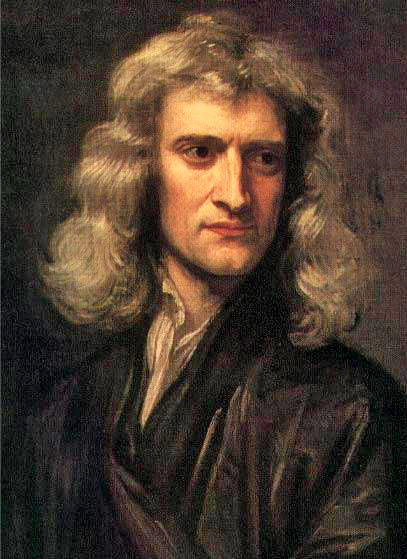
\includegraphics[scale=.9]{newton.jpg}
\end{figure}

\begin{center}
    \textit{To explain all nature is too difficult a task\\
    for any one man or even for any one age.\\
    'Tis much better to do a little with certainty\\
    and leave the rest for others that come after you.}\\
    	$\sim$Isaac Newton
\end{center}

\newpage
\begin{spacing}{1.0}
\tableofcontents
\end{spacing}

\newpage
\subsection*{Mission Statement}
\textit{Newton’s Notebook: The Haverford School STEM Journal} is designed to enhance the interests, talents, and achievements of individuals in mathematics and science and to promote the work of those most passionate about these disciplines. The following articles were written by members and friends of the Haverford community and edited by the \textit{Notebook staff}. We hope these articles inspire readers to further discover the universally beautiful realm of STEM exploration. 
\subsection*{Staff}
{\centering{}
    \textbf{Editor-in-Chief:} Alexander Greer '20
    \\
    \textbf{Assistant Editors:} Gary Gao '21, Mitav Nayak '22, Safa Obuz '21, Shibo Zhou '22
    \\
    \textbf{Designer-in-Chief:} Alexander Greer
    \\
    \textbf{Faculty Advisor:} Dr.\ Mark Gottlieb
    \\}
\subsection*{Featured Polymath: Richard Phillips Feynman (1918-1988)}
Richard Phillips Feynman was an American theoretical physicist known for his work on quantum mechanics, quantum electrodynamics, and particle physics. Born in Queens, New York, in 1918, Feynman excelled in math and science in high school. He attended the Massachusetts Institute of Technology and graduated with a bachelor’s degree in physics in 1939. In early 1943, Feynman was recruited by Robert Oppenheimer to work as a researcher on the Manhattan Project developing the atomic bomb. Soon after his work, Feynman took up a position as a physics professor at Cornell University. There he developed Feynman diagrams, a system of visually representing mathematical expressions describing the interaction of subatomic particles. In 1951, Feynman took up a position at the California Institute of Technology after taking a year-long sabbatical in Brazil. At Caltech, Feynman explored superfluidity and superconductivity, as well as conceiving the possibility of quantum computers. In the early 1960’s, Feynman produced \textit{The Feynman Lectures on Physics}, a lecture series outlining undergraduate physics concepts still used by university students to this day. In 1965, Feynman and two colleagues were awarded the Nobel Prize in Physics for their work on quantum electrodynamics. Feynman’s contributions to the advancement of human knowledge are innumerable, and his legacy as one of the world’s most-renowned scientists lives on. 
\newpage

% Begin the pure math section
\addcontentsline{toc}{part}{Pure Mathematics}
\nnimagepage{2020_Pure_Math_Section_Title.pdf}

\nnwallpaper{2020_Pure_Math_Page_Border.pdf}
\def\currentTitleWallpaper{2020_Pure_Math_Title_Page_Border.pdf}

\nnarticleheader{Gabriel’s Horn Paradox}{Mitav Nayak, Haverford '22}
\noindent
\textbf{Introduction}

	Perplexing yet intriguing, “Gabriel’s Horn” is a geometric shape formed by rotating the graph of $f(x)=\frac{1}{x}$ about the x-axis that has fascinated mathematicians for centuries. Evangelista Torricelli, an Italian mathematician and physicist, was the first to examine the shape during the 1600s. Torricelli studied under Galileo, and gained fame for his development of the barometer. Furthermore, Torricelli worked with infinite series, contributing toward the proof of the sum for the telescoping series. He was a prominent mathematical figure in the seventeenth century, and his work surrounding Gabriel’s Horn sparked debates surrounding the nature of infinity in the years after his death.

	Gabriel’s Horn – also known as Torricelli’s Trumpet – is a figure with a finite volume but an infinite surface area. In other words, if a painter was tasked with filling the horn with paint, he would need a finite amount of paint. However, if the painter was tasked with painting the entire inside or outside surface, it would be impossible, as he would need an infinite amount of paint. This paradox, known as the painter’s paradox, can be shown by solving for both the volume and surface area of the figure.
\\
%add first image here
\renewcommand{\thefigure}{1}
\begin{figure}[h!]
  \begin{center}
    
\includegraphics[scale=.25]{nayak_horn}
    \caption{Gabriel's Horn}
    \label{fig:1} 
  \end{center}
\end{figure}

\newpage
\noindent
\textbf{Mathematical Explanation}

	Consider the graph $f(x)=\frac{1}{x}$ (Figure 2). Now, consider this graph on the interval $[1,\infty)$ rotated about the x-axis (Figure 3).
	
\renewcommand{\thefigure}{2}
\begin{figure}[h]
  \begin{center}
    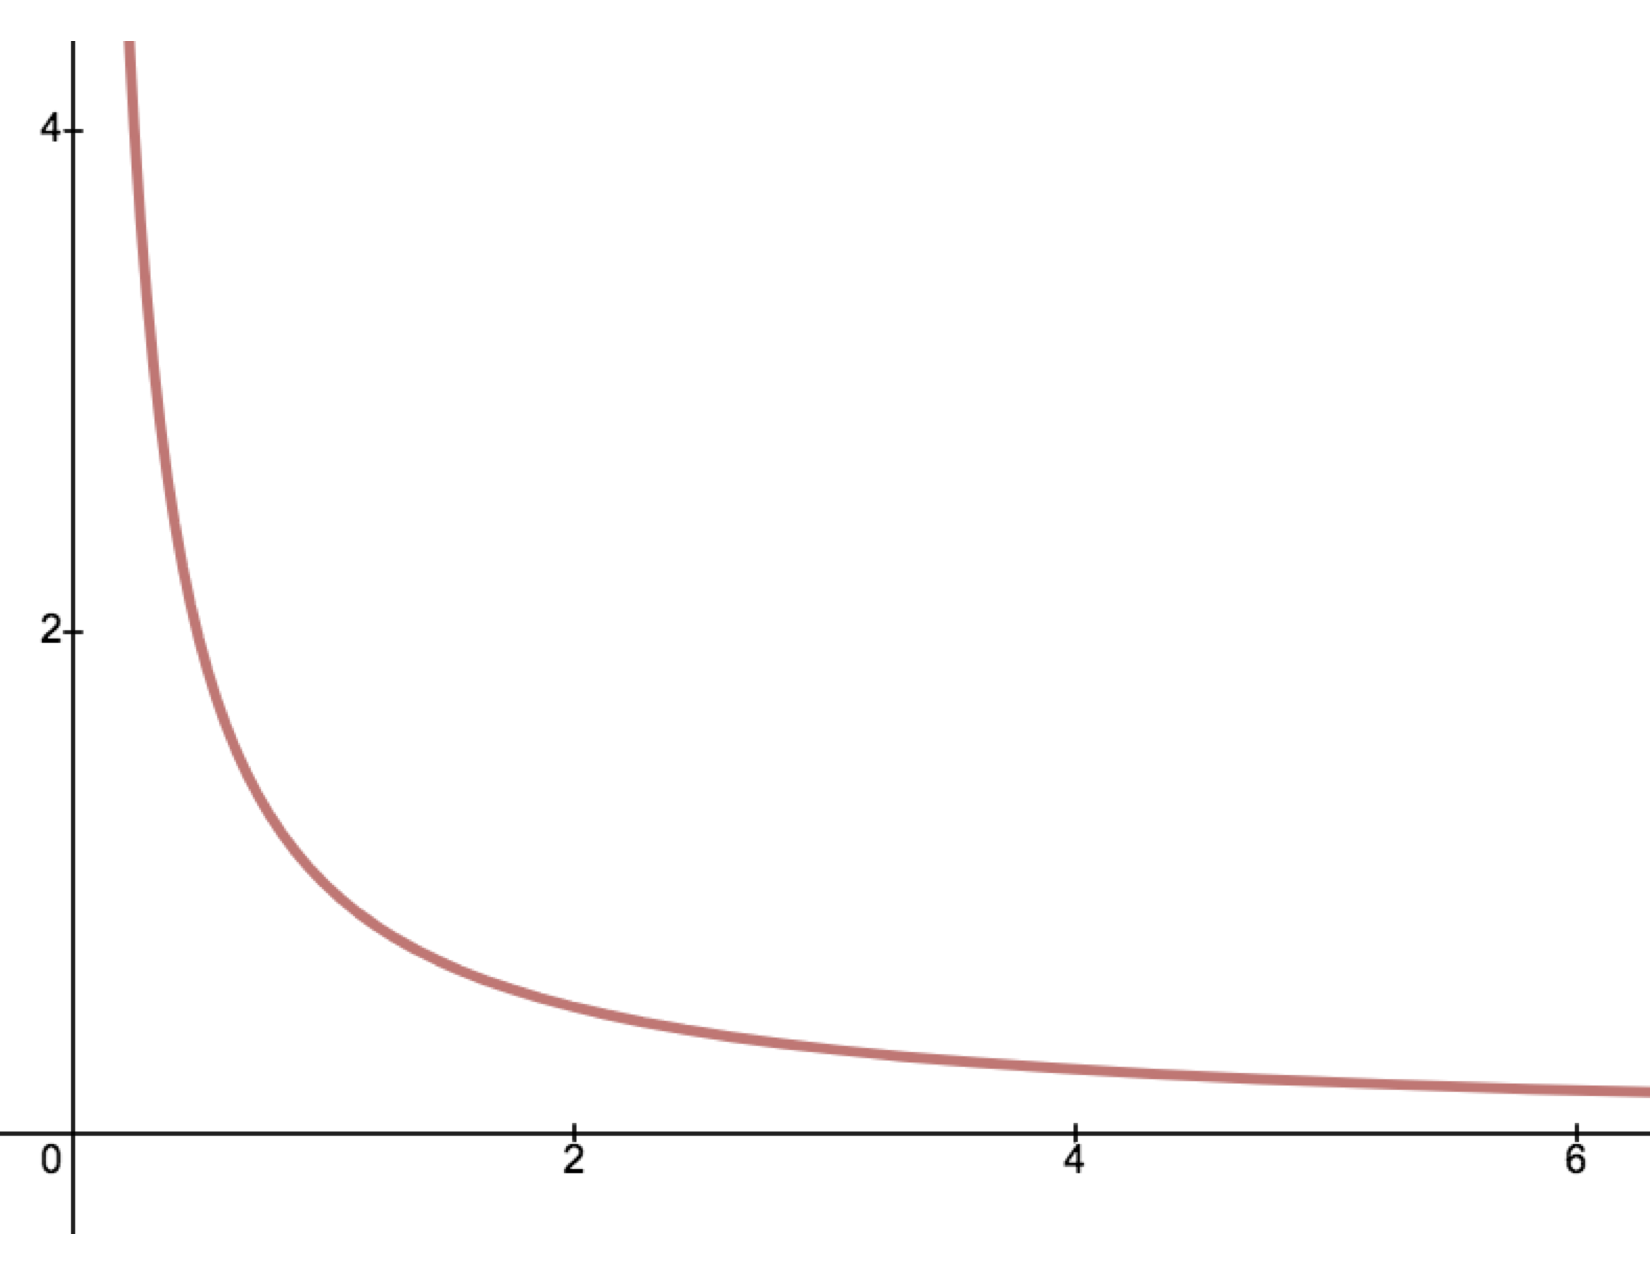
\includegraphics[scale=.3]{nayak_graph_1}
  \end{center}
  \caption{Graph of $f(x)=\frac{1}{x}$}
  \label{fig:2}
\end{figure}

\renewcommand{\thefigure}{3}
\begin{figure}[h]
  \begin{center}
    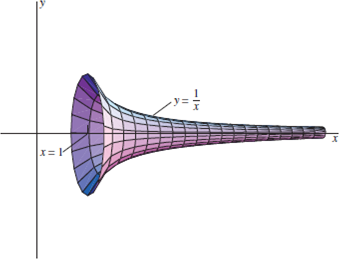
\includegraphics[scale=1]{nayak_graph_2}
  \end{center}
  \caption{Graph of $f(x)=\frac{1}{x}$ on the interval $[1,\infty)$ rotated about the x-axis}
  \label{fig:2}
\end{figure}

\noindent
\textbf{Part I: Solving for Volume}

The standard equation used in calculus for the volume of a curve rotated about the x-axis is: 

\begin{center}
$V=\pi\int_a^b((f(x))^2dx$
\end{center}

In this case, $a=1$, $b=\infty$, and $f(x)=\frac{1}{x}$, so the equation will be: 

\begin{center}
$\pi\int_1^\infty(\frac{1}{x})^2dx=\pi\lim_{b \to \infty} f(x)\int_1^b(\frac{1}{x})^2dx$
\end{center}

We can now solve the improper integral:
\[\pi\lim_{b \to \infty}\int_1^b(\frac{1}{x})^2 dx
= \pi\lim_{b \to \infty}[-x^{-1}]\bigg|_1^b
= \pi\lim_{b \to \infty}[(-\frac{1}{b})-(-\frac{1}{1})]
= \pi \cdot 1
= \pi
\]

Therefore, the volume of the figure is equal to $\pi$. Using the painter example, we can see that he must use $\pi$ cubic units of paint to fill the horn.

	\noindent
	\textbf{Part II: Solving for Surface Area}
		
	We can use another standard calculus formula to solve for the surface area of the figure: 

\begin{center}
$2\pi\int_a^bf(x)\sqrt{1+(f'(x))^2}dx$
\end{center}

Plugging in the known values, $a=1$, $b=\infty$, $f(x)=\frac{1}{x}$, and $f'(x)= -x^{-2}$, we get: 

\begin{center}
$2\pi\int_1^\infty\frac{1}{x}\sqrt{1+(\frac{-1}{x^2})^2}dx=2\pi\int_1^\infty\frac{1}{x}\sqrt{1+\frac{1}{x^4}}dx$
\end{center}

We know intuitively that $\sqrt{1+\frac{1}{x^4}}$ is always greater than 1, so we can say:

\begin{center}
$2\pi\int_1^\infty\frac{1}{x}\sqrt{1+\frac{1}{x^4}}dx>2\pi\int_1^\infty\frac{1}{x}\cdot1dx$
\end{center}

We now solve the improper integral of the second equation:
\[
2\pi\int_1^\infty\frac{1}{x} \cdot 1dx
= 2\pi\lim_{b \to \infty}\int_1^b\frac{1}{x}dx
= 2\pi\lim_{b \to \infty}[\ln{|x|}]\bigg|_1^b
= 2\pi\lim_{b \to \infty}[\ln{|b|}-\ln{|1|}]
= 2\pi\lim_{b \to \infty}[\ln{|b|}]
\]

Since this limit approaches infinity, and since the equation for the surface area of the figure is greater than this limit, the figure’s surface area is also infinite. Therefore, a finite amount of paint will always be unable to cover the full surface of the horn.

\noindent
\textbf{Conclusion}
	
	It is clear why Torricelli’s discovery generated debate among the mathematical community. Many brilliant minds of the time – including Italian astronomer Galileo Galilei, English philosopher Thomas Hobbes, English mathematician John Wallis – struggled with the paradox, as they believed it challenged their ideas of the nature of infinity. After all, how could a figure have a finite volume, and yet have an infinite surface area? Torricelli titled his discovery “Torricelli’s Trumpet,” and it later became better known as Gabriel’s Horn — a reference to the archangel Gabriel. In the Hebrew Bible, the archangel blows his horn on Judgement Day and is related to the divine and the infinite.

\newpage

\nnarticleheader{Impartial Games and the Sprague-Grundy Theorem}{Gary Gao, Haverford '21}
\noindent
\textbf{Overview -- Impartial Games}

	In combinatorics, there has been a field that studies the processes and outcomes of games -- Game Theory. And among many games, the impartial games are the most fundamental ones to study. To highlight the point of this topic, I can say that this particular section of the impartial game reveals how millions of games work, which means some generalization can provide us with many intuition and insights about game strategies.
	\begin{definition}
		An impartial game is a game in which the allowable/possible moves depend only on the position at which the game is and not on which of the players is currently moving, and where the payoffs are symmetric.
	\end{definition}
	
	In other words, the only difference between player 1 and player 2 (or other players) is that player 1 goes first. The game is played until a terminal position is reached, in which an additional move is not possible. Then one of the players is declared the winner and the other the loser. Furthermore, in order to fully understand the strategies of the game, impartial games are played with perfect information and no chance moves, meaning all information about the game and operations for both players are visible to both players, and all players play their best possible moves usually. \textbf{Our goal is to determine what are the best or the most favorable strategies for each player at each position of the game.} More specifically, which player has the winning strategy at the moment if the game proceeds to a certain situation? Or if the game can be forced to a draw?

\noindent
\textbf{The Nim Game}

\noindent
\textbf{An Intuitive Example}

Here is a famous and simple game:
		\begin{problem}
			There is a pile of 100 stones on the ground. Two players, called Alice and Bob, play the following game: Starting with Alice, each player can and must take away 1, 2, or 3 stones. At the end, the player who takes away the last stone wins. Who has the winning strategy? And what is his/her strategy?
		\end{problem}
		\begin{solution}
			The strategy is not hard to spot. We can see that there is a nice way for Bob to counter a move made by Alice. Since one can only take 1,2, or 3 stones, it reminds us that we can utilize the divisibility of 4. Whenever Alice takes $n$ stones away, bob can then take $(4-n)$ away so that after a round, the number of stones left is still divisible by 4 (since $4|100$). Therefore, Bob can secure the last stone since his move would always be reducing the number of stones to a multiple of 4.
		\end{solution}
	
	\noindent
	\textbf{What Is A Nim Game?}
	
		\begin{definition}
		A Nim game is a game in which two players take turns removing objects from distinct piles. During each move a player must remove at least one object, and the player can remove any number of objects from the same pile. 
		\end{definition}
		
		We can see that a definition for the most general Nim game is similar to the example we touched on earlier. But the key element here is that one player can remove \textbf{any} amount of objects from a pile. Now there is a question: what is the point of the game if all stones may be removed at once? The answers is: yes, the game with only 1 pile is trivial now. But what if we have multiple piles?
		\begin{problem}
			There are two piles of stones. The first one has $a$ stones and the second one has$b$. Alice and Bob plays the Nim game on these two piles starting with Alice. Who has the winning strategy, and why?
		\end{problem}
		To fully understand the mechanism and lay a foundation for further exploration, we now introduce a method.
	
\noindent	
	\textbf{Winning And Losing Positions}
	
		To simplify the problems, we consider that the game has a winning-losing outcome for sure.
		\begin{definition}
			A winning position is a position of the game at which the player making the subsequent move has a winning strategy. A losing position is a position of the game at which the player making the subsequent move will not have any strategy to win, which means that (one of) the player's opponents has a winning strategy.
		\end{definition}
		Now we try to find some nice properties about the game when there are 2 players.
		\begin{theorem}
			In a game with 2 players, a position is winning if and only if the player making a move can change the situation to a losing position after he moves.
		\end{theorem}
		This is obvious. If player 1 changes the game to a losing position, then player 2 will definitely lose (so that player 1 wins), making the original position a winning position. In all the following explanations and solutions to the problems we refer ``winning" and ``losing" positions as winning or losing for Player 1. And a winning position is denoted by ``$+$" and a losing one by ``$–$" for simplicity.
		
\noindent
	\textbf{Solution to 2 Pile Nim Games}
	
		\begin{solution}
			Denote $(a,b)$ as the case where the two starting piles have $a$ and $b$ stones respectively.\\
			\indent First notice that by an extension of the definition $(0,0)$ is a losing position because before this step Bob already won. Therefore, we use the following method to fill out a table: place $(0,0)$ at the top left. As $a$ or $b$ increases, we put a ``-" in the cell $(a,b)$ if and only if there is no other ``-" signs to the left or top of the cell.
			\begin{center}
			\begin{tabular}{|c|c|c|c|c|c|c|}
			\hline
			$(a,b)$&0&1&2&3&4&...\\
			\hline
			0&-&+&+&+&+&...\\
			\hline
			1&+&-&+&+&+&...\\
			\hline
			2&+&+&-&+&+&...\\
			\hline
			3&+&+&+&-&+&...\\
			\hline
			4&+&+&+&+&-&...\\
			\hline
			...&...&...&...&...&...&...\\
			\hline
			\end{tabular}
			\end{center}
			
			Then we can clearly see that it is a losing position for Alice if and only if the two starting piles have the same amount of stones. We can verify and prove this in two ways. One is by some simple induction. The other one is that whenever Alice removed some stone in pile 1, Bob imitates that move in pile 2 so that he can secure the victory.
		\end{solution}
		\noindent
	\textbf{Solution to The General Nim Game}
	
		\begin{problem}
			There are $n$ piles of stones. The $k$th pile has $a_k$ stones ($1\leq k\leq n$). Alice and Bob plays the Nim game on these n piles starting with Alice. Who has the winning strategy, and why?
		\end{problem}
		We can first try to explore with the case where $n=3$. By filling out some tables with different $(a_1,a_2,a_3)$, we can certainly find some patterns but they do not appear in a nice way. We can try to obtain a pattern via brute force through all triplets of numbers of stones but the pattern do not have any apparent recursion. (It is also hard because the table would be 3-dimensional). However, it is possible for us to see that in most cases, Alice will still win. We can also obtain some small cases where the starting position is a losing one for Alice:\\
		WLOG, organize them in the way that $a_1 \leq a_2 \leq a_3$
		\begin{center}
		$(0,1,1),(0,2,2),(0,3,3),...$\\
		$(1,2,3),(1,4,5),(1,5,6),...$\\
		$(2,4,6),(2,5,7),(2,8,10),(2,9,11),(2,12,14)...$\\
		$(3,4,7),(3,5,6),(3,8,11),(3,9,10),(3,12,15)...$\\
		$(4,8,12),(4,9,13),(4,10,14),(4,11,15),(4,16,20),...$\\
		\end{center} 
		Using intuition, we can begin to see that the triplets have some characteristics of cycles of 1,2,4,..., the powers of 2. Thus, we explore them in a way related to binary expressions of integers.\\
		\begin{definition}
			Nim Plus $a \oplus b$ for integers $a,b$ is defined as the bitwise exclusive or operation on the binary expressions of the number $a$ and $b$.
		\end{definition}
		The exclusive or operation means that $1 \oplus 1 = 0 \oplus 0 = 0, 1 \oplus 0 + 0 \oplus 1 = 1$. We do this operation on every digit of the binary expression of 2 numbers independently and combine them together. For example, $113=(1110001)_2, 189=(10111101)_2$
	
		\begin{center}
			\begin{tabular}{ccccccccc} 
			&1&0&1&1&1&1&0&1\\
			$\oplus$&&1&1&1&0&0&0&1\\
			\hline
			&1&1&0&0&1&1&0&0
		\end{tabular}
		\end{center}
		So $113 \oplus 189 = (11001100)_2 = 204$. Also notice that the Nim sum obey the associative and the commutative laws, and that $x \oplus y = 0$ if and only if $x = y$.
		\begin{theorem} 
		In a Nim game using $n$ piles with $a_1, a_2, a_3, ... , a_n$ stones in the 1st, 2nd, 3rd, ..., nth pile respectively, the starting position is a losing one for the first player if and only if $a_1 \oplus a_2 \oplus a_3 \oplus...\oplus a_n$ = 0.			
		\end{theorem}
		\begin{proof}
		Let a situation be $X = (x_1,x_2,...,x_n)$. Let a situation after doing one move on $X$ be $Y = (y_1,y_2,...,y_n)$. Let $p = x_1 \oplus x_2 \oplus... \oplus x_n$, $ q = y_1 \oplus y_2 \oplus ... \oplus y_n$. Let $x_k$ and $y_k$ be the number of stones in the $k$th pile (the one that is changed) before and after the move.  By definition $x_i = y_i$ except when $i=k$. Therefore:
		\begin{align}
		\nonumber q &= y_1 \oplus y_2 \oplus ... \oplus y_k \oplus ... \oplus y_n\\
		\nonumber   &= x_1 \oplus x_2 \oplus ... \oplus x_{k-1} \oplus y_k \oplus ... \oplus x_n\\
		\nonumber   &= x_1 \oplus x_2 \oplus ... \oplus x_{k-1} \oplus y_k \oplus (x_k \oplus x_k) \oplus ... \oplus x_n\\
		\nonumber   &= x_1 \oplus x_2 \oplus ... \oplus x_k \oplus ... \oplus x_n \oplus x_k \oplus y_k\\
		\nonumber   &= p \oplus x_k \oplus y_k
		\end{align}
		
		\indent We first prove that if $p=0$ then after a move $q\neq0$. If $p=0$, $q=x_k \oplus y_k$, which cannot be zero because $x_k \neq y_k$.\\
		\indent Then, if $p\neq0$, we prove that there exist some number $a \leq \max\{x_1,x_2,...,x_n\}$ such that for some $x_k \leq a$, $q = p \oplus x_k \oplus a = 0$ (which means we reduce the kth pile to $a$ stones). In fact, if we let $a = x_1 \oplus x_2 \oplus ... \oplus x_{k-1} \oplus x_{k+1} \oplus ... \oplus x_n$, it satisfies the condition that $q = 0$. We just have to prove that it is possible for us to find a $k$ such that $x_1 \oplus x_2 \oplus ... \oplus x_{k-1} \oplus x_{k+1} \oplus ... \oplus x_n \leq x_k$. Notice that this $a$ is equivalent to $p \oplus x_k$. Let's find the leftmost nonzero digit of the binary representation of $a$ to be the $d$th digit from the right. Then, there must exist a $x_k (1\leq k\leq n)$ such that its $dth$ digit from the right is nonzero (which mean it is 1). This is because if all of the $x_i$ have zero on that digit, $a$ must be zero, making a contradiction.\\
		\indent Therefore, we've established that if $p=0$ then $q\neq0$ and vice versa, establishing a connection between two types of positions. Since empty piles are defined to be losing for the first player, we can easily see by induction that the theorem is proved.
		\end{proof}
		Thus ends our solution to the problem of Nim Games.

\noindent
\textbf{The Sprague-Grundy Theorem}

\noindent
	\textbf{History}
	
		The Sprague-Grundy theorem and its proof contains the main results of a theory discovered independently by German Mathematician Roland. P. Sprague (1935) and English Mathematician Patrick. M. Grundy (1939). Therefore the theorem is named after both of them.
		
		\noindent
	\textbf{Theorem Statement}
		\begin{theorem}
			\textbf{Sprague-Grundy Theorem:} Every impartial game under the normal play convention is equivalent to a nimber (which is a Nim Game with 1 single pile).
		\end{theorem}
		The normal play convention here refer to the common and standard ways to determine a game's winner; e.g. \textbf{preventing the other player from being able to move}, being the first player to achieve a target, having the highest value of something, etc. Therefore, in our case, the theorem states that every impartial game is just equivalent to the Nim game we just solved. The proof of the theorem is very complicated and abstract thus it would not be given explicitly here. Intuitively, the proof uses induction to classify every possible position of the game by assigning it a number $a$, indicating that the position is equivalent to a pile of $a$ stones in a Nim Game. Then it is also possible to show that the Nim Game is the \textbf{same} even if you allow arbitrary \textbf{adding of stones} to a pile as a possible move (as long as there are some limitations to ensure that the number of stones will reduce to zero). For instance, if a situation can go to situations that correspond to 1,2,3,... stones in a pile after a move, the situation will be equivalent to a 0-pile (the losing position for the first player by definition). 
		\noindent
	\textbf{Remarks}
	
		 Although the theorem does not provide any specific way to map the equivalence or conversion, it still offers some very helpful insights in solving these problems. Basically, when we encounter any impartial game, we can try to convert it to a Nim Game. 
		 \noindent
	\textbf{An Example}
	
		\begin{problem}
			Suppose we have a chocolate bar composed of small squares of chocolate that form a triangle. There is a square with bad taste somewhere in the middle. Alice and Bob alternate to cut off and eat a rectangular piece along the horizontal/vertical grid (only one straight cut allowed each time) that does not contain the bad square. Who has the strategy to force the other player to eat the bad square finally?
		\end{problem}
	
		\begin{solution}
			With the idea of Sprague-Grundy theorem, we can try to come up with a nice way to link the actual game to some Nim Game. Such a construction can be found with the help of a diagram (red cell indicating the bad square):\\

\begin{figure}[h]
  \begin{center}
    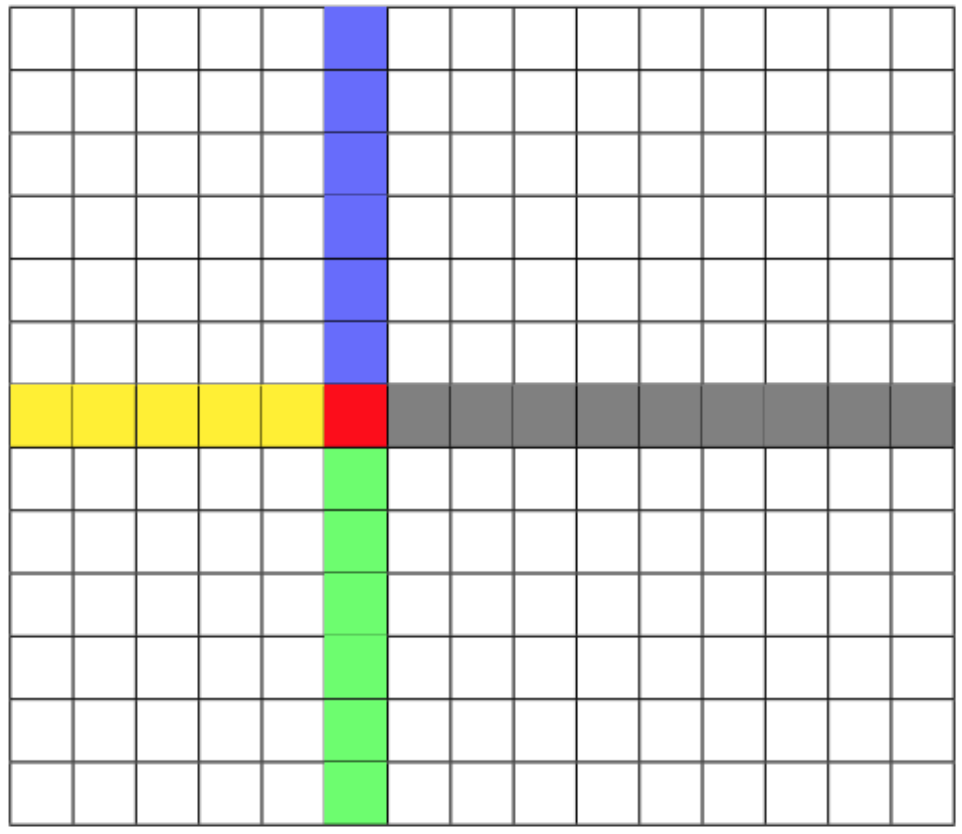
\includegraphics[scale=.6]{gao_diagram}
  \end{center}
\end{figure}

			\indent Then we can see that each move is equivalent reducing one of the four strips (blue, gray, yellow, and green) to any nonnegative amount of squares by making one horizontal/vertical cut. This game is exactly the same with a Nim Game with 4 piles. Therefore, if the four strips have $x_1,x_2,x_3,x_4$ squares respectively, Bob will win if and only if $x_1 \oplus x_2 \oplus x_3 \oplus x_4 = 0$.
		\end{solution}
		\noindent
	\textbf{Summary}
	
		The study of impartial games contributes to the combinatorial game theory field and broadens our understanding in all sorts of non-impartial games that humans have created (chess, checkers, pokers, etc) as well. We can see that the buildup to Sprague-Grundy theorem is relatively long, since solving the Nim Game completely requires some new lemmas and definitions. The formulation of the theorem is concise but also links all impartial games together, which shows most charming element of combinatorics: It is a study dedicating to the conversion very broad, abstract, and verbal problems and objects to organized, rigorous, and powerful results and theorems in mathematics.

\newpage

\nnarticleheader{Pigeonhole Principle}{Will Vauclain, Haverford '19}

In the field of Discrete Mathematics, there is a theorem commonly known as the
Pigeonhole Principle. In its most basic form, it states ``if you have $n$
holes and $n + 1$ pigeons, then there must be two pigeons in the same hole.''
While this statement seems obvious, it is useful in proving a wide variety of
theorems. In this article, we will prove two: the first purely theoretical and
the second a practical application in computer science.

\textit{Theorem 1: In any geometric progression 1, $a$, $aa$, $a^3$, etc.,
outside of the first term 1, there is still another term $a^t$ which is
congruent to the unity relative to the modulus $p$ when $p$ is prime relative
to $a$; and the exponent $t$ is $< p$.}

This theorem appears in Gauss's
\textit{Disquisitiones Arithmeticae}, and his main argument relies upon the Pigeonhole
Principle. To start with, we should rephrase the question in more
understandable terms. Gauss claims that given two numbers $a$ and $p$ which are
relatively prime (i.e. they share no common factors besides 1), there exists
some number $a^t$ such that $a^t - 1$ is divisible by $p$, and $1 \leq t < p$.
For example, for $a = 3$ and $p = 2$, $3^1 - 1 = 2$, which is divisible by 2,
and $1 \leq 1 < 2$.

\noindent
\textbf{Proof:}

Let us first consider all possible remainders when dividing
$a^t$ by $p$. Since $a$ is not divisible by $p$ (otherwise they would share a
common factor of $p$), $a^t / p$ can only have a remainder between 1 and $p -
1$. Suppose that there are no values of $t$, $1 \leq t < p$, such that $a^t -
1$ is divisible by $p$, which means that no $a^t$ has remainder 1 (we will show
why this is impossible, thus proving that there must exist such a $t$). This
means that there are $p - 2$ possible remainders for $a^t / p$ (any value from
2 to $p - 1$). Since there are $p - 1$ possible values of $t$, by the
Pigeonhole Principle, there must be two $t$'s such that $a^t / p$ has the same
remainder $r$. Let the larger one be $u$ and the smaller one be $v$. Since
$a^u$ and $a^v$ both have the same remainder when divided by $p$, $a^u - a^v$
must be divisible by $p$. $a^u - a^v = a^v(a^{u - v} - 1)$. Since we know $a^v$
cannot be divisible by $p$, $a^{u - v} - 1$ must be divisible by $p$, and since
$u > v$, we know $1 \leq u - v < p$. This contradicts what we assumed earlier:
that there is no such value of $t$. Therefore, there must always be some $t$,
$1 \leq t < p$, such that $a^t - 1$ is divisible by $p$.

\textit{Theorem 2: It is impossible to create a lossless algorithm
which compresses each input file to a smaller output file.} 

This theorem has practical applications pretty much everywhere computers are used. A lossless
compression algorithm is any compression algorithm which allows the input to be
perfectly reconstructed from the output (think of a .zip file, where
files are reconstructed perfectly from their compressed form). The theorem states that every
lossless compression algorithm must have some file  it cannot compress into a smaller size.

\noindent
\textbf{Proof:}

For simplicity, we will assume that every input file has
exactly $k$ bits of information, for some $k$ (in other words, it can be
represented as a binary number with $k$ ones and zeros). This simplifying
assumption turns out not to matter, as we will see later, but it makes the math
considerably easier. Let us first figure out how many possible output files
there are (i.e. how many possible strings of ones and zeros with length less
than $k$). The number of strings of ones and zeros of length $p$ turns out to
be equal to $2^p$, since for each digit you can pick either a 1 or a 0. Thus the
number of strings of length less than q is $2^0 + 2^1 + \ldots + 2^{k - 1}$.
This is a finite geometric series, so its sum is equal to $\frac{2^{k - 1 + 1}
- 1}{2 - 1} = 2^k - 1$. Since there are $2^k$ files with exactly $k$ bits of
information, and only $2^k - 1$ files with less than $k$ bits of information,
by the Pigeonhole Principle any compression algorithm which makes every file
smaller must map two files to the same output, but this would mean that the
compression algorithm is not lossless, since you would not be able to tell
which of the two input files was used to create the output file. Here we see
how our simplifying assumption doesn't matter. If we consider files of every
size, then some of the smaller output files would map to smaller input files,
which just makes the lack of available output files even worse. Thus, every
lossless compression algorithm must fail to make some of its inputs smaller.

\newpage

\nnarticleheader{Four Proofs of Euler's Identity}{Elise Kait, Baldwin '21}


\newpage

% Begin the philosophy of math section
\nnwallpaper{2020_Philosophy_Page_Border.pdf}
\def\currentTitleWallpaper{2020_Philosophy_Title_Page_Border.pdf}

\addcontentsline{toc}{part}{Applied Mathematics}
\nnimagepage{2020_Philosophy_Section_Title.pdf}

\nnarticleheader{Foundations of Mathematics}{Dr. Mark Gottlieb, Haverford Faculty}
\noindent
\begin{quotation}
\textit{The science of pure mathematics ... may claim to be the most original creation of the human spirit.}
\begin{flushright}
Alfred North Whitehead
\end{flushright}
\end{quotation}
\noindent
\textbf{Introduction}

     Although we are all familiar with basic mathematical ideas and operations, most of us would be at a loss if we were asked to define mathematics, to say what mathematics "really is".  We know, for example, that mathematics studies numbers, shapes, and patterns.  But what is a number?  Although numbers seem to be important in nearly all practical situations, a number does not seem to be a material object.  For example, unlike physical objects, numbers do not seem to undergo change.  Physical things age and, eventually, fall apart.  Numbers do not.  Whatever properties a number has, it seems that it has always had them and always will.  For example, the number 7 is prime because it has no whole number factors other than 1 and 7.  That makes it different from 6, for example, because 6 = 2 x 3.  It seems clear that 7 will always be prime and that 6 never will be. 
      
     
     Numbers, unlike physical objects, are not things we perceive by means of the senses of  sight, hearing, or touch.  In a similar way the triangles, circles, and squares that we study in geometry, if we think about it carefully, are not perceived by the senses, either.  In this case we feel more confident in asserting that these objects belong to the "real world" of space.  For example, we may feel that we can draw a triangle on a blackboard or construct a circle on a piece of paper using a compass.  If we think carefully about this, however, we realize that, no matter how accurately we draw our picture, it will, at least in some small respect, remain only an imperfect copy of what we imagined.  In point of fact, no one can ever draw a triangle, circle, or square.  Nevertheless, like numbers, geometrical objects seem to have unchanging properties.  For example, the sum of the measure of the angles of a triangle is always $180^{\circ}$.\footnote{Interestingly, we might be inclined to doubt this were we restricted to making measurements with a protractor, since we would almost certainly measure the sum to be different from exactly $180^{\circ}$. }
     
     We can now see that neither numbers nor geometrical figures are material objects, but what about patterns and relations?  Like numbers and shapes, patterns and relations seem to be very real features of the world.  And, just like numbers, they do not seem to be material objects.  What is going on here?  Mathematics seems to be the study of certain kinds of things that, while very much real, do not belong to the physical world.  At first, it may seem rather puzzling that there appear to be real things that are not physical, but the fact that we can acquire mathematical knowledge challenges our belief that all real things are physical.  It may surprise you that mathematicians themselves are deeply puzzled by this problem, as well.  

\noindent
\textbf{Realism}

     Until the beginning of the nineteenth century most mathematicians believed that they were studying non-physical objects that were unchanging and eternal.  They believed that, somehow, the human mind could "grasp" mathematical truths by directly "seeing" them, just as we "see", for example, that 7 + 5 = 12.  The view that mathematics is made up of eternal truths about unchanging objects is an ancient idea.  It goes back to the sixth century B.C. and is associated with the teachings of the Greek religious brotherhood known as the Pythagoreans.  According to these men, their founder, Pythagoras, had taught that the real world is not the way it seems to the senses, but is actually governed by invisible mathematical relationships.  The Pythagoreans seem to have made the discovery that the basic intervals of the Western musical scales, for example, the octave or the fifth, are the result of dividing a stretched string into whole number ratios.  Cutting the string in half, for example, results in raising the pitch by one octave.  Cutting it in a ratio of 2:3 results in raising it by the major fifth (e.g., from middle C to the G directly above it).  These remarkable discoveries must have been awe-inspiring to the men who made them, for they showed that the universe obeys exact mathematical relationships.  This inspired them to hold mathematics in the highest esteem as the very basis of the universe.  Interestingly, the Pythagoreans later experienced profound dismay when it was discovered that there are numbers such as $\sqrt{2}$   that are not equal to any fraction, however large the denominator.
     
     Many scholars today regard Plato as the greatest and most influential of the ancient Greek philosophers.  As a young man he became acquainted with the teachings of earlier Greek thinkers, like the Pythagoreans, who believed that mathematics was the study of unchanging objects. Throughout his many writings, he expressed the view, quite similar to that of the Pythagoreans, that the world as it appears to the senses is not completely real.  Instead, beyond the world of the senses lies the world of Ideas or Forms which are perfect and unchanging.  For example, Plato argued that, while any particular tree was always changing and gradually decaying, the concept or Form, "Tree", always remained the same.  Scholars often refer to Plato's view as his "Theory of Forms", and numbers, shapes, and other mathematical objects are among the Forms.  Mathematicians who share Plato's view are, naturally, known as Platonists or mathematical realists.
     
    Realism appeals to mathematicians for a number of reasons.  It seems to give mathematics a special significance and dignity among the sciences.  First, as we have mentioned, mathematics seems to be special mainly because it is the only subject that studies unchanging objects.  Platonists believe these objects have always existed and will always exist.  Furthermore, because mathematical facts come from the properties of  these objects, no human being can alter them.  Mathematical truth, according to the Platonist, is objective  and independent of human minds.  Mathematical research, just like research in the sciences, is the attempt to discover, not to create, new mathematical facts and ideas.  Finally, mathematical ideas seem to be totally clear and distinct, unlike the concepts used in other subjects, like biology or history.  Realists explain this clarity by pointing to the fact that mathematical objects are not made up freely by the human mind, but have a perfect form in and of themselves.  Although they may not be quite clear about it in their own minds, it is probably fair to say that most mathematicians engaged in theoretical research today are realists, at least in spirit.  Interestingly, however, very few eminent mathematicians in recent times have actually called themselves realists.  Notable exceptions include Kurt Gödel, perhaps the greatest logician of the twentieth century, and the French mathematician René Thom, who helped to establish a branch of mathematics called \emph{chaos}.  
    
    If Platonism expresses so many common beliefs about mathematics, why have so few mathematicians been willing to call themselves Platonists?  Platonism is an appealing viewpoint for mathematicians, but it is very difficult to justify the idea that mathematical objects have no connection to the material world.  For example, if mathematical objects exist in a non-physical world, how do our brains, which are obviously physical, ever come into contact with them?  How does the number 7 or a right triangle get inside my brain so I can think about it?   Perhaps in my brain there are only numerals, or symbols for numbers.  But, then, how do these numerals connect to numbers?  This is a mystery.  It seems that numbers must be somehow connected with the physical world if we are to be able to understand mathematics (or, for that matter, to teach it to others).\footnote{On this point see R. Hersch, \textit{What is Mathematics, Really?}.}  In science, particularly in physics, mathematical equations are used to represent events and relationships in the material world, what physicists call "laws of nature."  If mathematical objects do not belong to the physical world, it is very difficult to see how or why physical laws should be mathematical.  Along these lines, the physicist Eugen Wigner once remarked that mathematics was "unreasonably effective" in physics.  

\noindent
\textbf{Logicism}

     There is one further puzzle that Platonism creates but doesn't solve.  If mathematical objects exist in a non-physical place, and if we are able to recognize mathematical truths by directly "seeing" them, why do mathematicians find it necessary to go through careful reasoning or proof  in order to be sure they are reaching correct conclusions?  All of modern mathematics is based upon the idea of  justifying our conclusions by going back to a set of very basic assumptions, called axioms or postulates.  Clearly, if we are to prove something, we have to start somewhere.  If we had no background knowledge whatsoever, we could never reach any conclusions.
     
     For example, supposing we know that all birds are warm-blooded and that  penguins are birds, we can prove that penguins are warm-blooded.  We can depict our reasoning process as follows:

\begin{center}
Assumption 1: All birds are warm-blooded. Assumption 2: All penguins are birds.

Conclusion: All penguins are warm-blooded.
\end{center}  
An example of a very simple mathematical argument is the following:
\begin{center}
Assumption 1: A = B. Assumption 2: B = C.

Conclusion: A = C.
\end{center}

Mathematicians call this pattern of reasoning the \emph{Transitive Property of Equality}.
In both of the cases above, the conclusion follows necessarily from the assumptions.  It is not possible for the assumptions to be true and the conclusion to be false.  It is time to introduce our first formal definitions.
\begin{dfn}
A \textbf{deductive argument} is any set of statements in which one statement, the conclusion, is marked off from the other statements.
\end{dfn}
\begin{dfn}
A \textbf{proof} is a collection of statements placed in an order such that the last statement, called the conclusion, follows from the truth of the other statements.  In mathematics, the conclusion is called a \textbf{theorem}.   Note that a deductive argument may or may not be a proof, since the conclusion may or may not follow logically from the other statements.
\end{dfn}
\begin{dfn}
A(n) \textbf{hypothesis} of  a deductive argument is an assumption or starting point of the argument.
\end{dfn}

The idea of building up mathematical knowledge by a chain of deductive arguments starting from axioms or postulates goes back to the ancient Greeks, who excelled in both logic and geometry.  The most important example of this way of doing mathematics is contained in the work of  Euclid, who brought together much of was known about geometry in a single book, the \emph{Elements}.  In this book Euclid identified a basic set of geometrical axioms (unproven assumptions)  from which every other result could be proven.  This was an extraordinary achievement and has exerted a tremendous influence upon all of mathematics, science, and philosophy in the Western world.  Interestingly, until the twentieth century, mathematicians did not succeed in building up arithmetic and algebra, which study numbers and number operations, from a set of simple axioms.  Today, there are still unresolved problems about how to accomplish this goal correctly.

     Some mathematicians, impressed by the power of logic and proof, have tried to solve the problems created by Platonism by arguing that mathematics is really just a collection of deductive arguments, starting from a set of basic, unprovable assumptions.  In other words, according to these mathematicians, mathematics is the same thing as careful reasoning or logic.  This viewpoint is called logicism.  Its most famous proponent  was the German philosopher Gottlob Frege, one of the creators of modern logic, which expresses deductive arguments using special symbols.  During the twentieth century, many mathematicians, wary of becoming Platonists, defended the position that mathematics is really logic, and many books about what is called mathematical logic were written.  Eminent philosophers, such as Bertrand Russell, W.V. Quine, and Rudolph Carnap, spent large parts of their careers developing systems of mathematical logic.  Despite these efforts, no one has ever been able to show how to express all of mathematics as pure logic.   It turns out that it is always necessary to bring in ideas that are not actually logical, but practical.
     
     We have to make sure, for example, that we don't end up in a muddle by talking about mathematical objects that can't really exist.  One of the main goals of the logicians mentioned above was to show that all the objects we work with in mathematics--numbers, spatial relationships, patterns--can be expressed in their most basic form as sets, or collections.  The study of sets was begun by the German mathematician Georg Cantor, who was especially interested in infinite sets.  Later in this book we will discuss how Cantor used the theory of sets to reach remarkable conclusions about infinite collections.  Let's make a few definitions pertaining to sets.
     
\begin{dfn}
A \emph{set} is any collection.  The members or \emph{elements} are the things that belong to the set.  We use the symbol $\in$ to indicate that a member belongs to a set.
\end{dfn}

We denote a set by using a variable symbol, usually a capital letter, and we represent that set by enclosing its elements within brackets.

\begin{exm}{1}
The set $\Re$ of real numbers can be represented by$\lbrace 1, 2.56, \pi, e, ...\rbrace$.  Here, the ellipsis ... means that the set has infinitely many members.
\end{exm}

\begin{exm}{2}
The set of all birds can be represented as B=$\lbrace$ my pet pigeon, the bald eagle in the zoo, ..., the University of Iowa mascot $\rbrace$.  Here the ellipsis replaces all the birds that are not written down (it would be a long list!).  Notice that a set does not have to contain numbers; it can have any members whatsoever.  This is a finite set.
\end{exm}

Bertrand Russell, one of the major proponents of logicism, recognized that there are sets that we can describe in words that simply make no sense.  Here is Russell's idea:  Some sets have the interesting property that they are \emph{members of themselves}.  For example, the set of \underline{all} sets is a set, so it is a member of itself.  As another example, consider the set T of all sets that contain more than 10 members.  This is an infinite set, and we can represent it as follows.
\begin{center}
$T=\lbrace\lbrace1,2,...11\rbrace,\lbrace1,2,...12\rbrace,...\rbrace$
\end{center}
 

Clearly T has more than 10 members, so T belongs to itself.  In our notation we write $T\in T$.  T is a set that contains itself as a member!  Obviously, this is not true of most sets.  For example, the set B of all birds above does not contain itself as a member; only birds belong to B, not sets.\\

     Now suppose we think about the set of all sets that are not members of themselves, like B.  Let's call these sets \emph{standard} sets\footnote{I borrow this term from S. Körner, \textit{Philosophy of Mathematics}, p. 45.} and denote the collection of all standard sets by S.  We can represent S as follows.
     \begin{center}
     S = $\{ B, \Re, \{1,2,3\},...\}$
     \end{center}

Here is Russell's question: Is S a standard set?  That is, is S a member of itself?  Well, if $S\in S$ , then S would seem to be standard, since it belongs to the set of standard sets, \underline{but} S would also seem to be non-standard, since it belongs to itself.  On the other hand, if $S\notin S$ , then S would seem to be standard, so $S\in S$  !  It looks like the following is true:

\begin{center}
$S\in S$ if and only if  $S\notin S$
\end{center}

It seems that S can neither belong to itself nor not belong to itself. What's going on here?

     This puzzle is known as \emph{Russell's Paradox}.  A logical paradox is a proof that has mutually contradictory conclusions.  Another famous logical paradox, which comes from the ancient Greeks, is called the \emph{Epimenides (or Liar) Paradox}.  Suppose a man says, "I am lying".  Is he telling the truth?  If he is, then he is lying, so he isn't telling the truth.  Conversely, if he isn't telling the truth, then he is telling the truth, since he is asserting that he is a liar.  His statement is paradoxical.
     
    Remember that the goal of the logicists was to show that mathematics is really just pure logic.  But there is nothing wrong with our reasoning when we reach a paradox.  In other words, logical thinking can lead to paradoxes.  On the other hand, we never seem to reach any paradoxes when we work with numbers, shapes, or patterns.  There are paradoxes in logic, but none in mathematics, so mathematics doesn't seem to be identical to logic.  In fact, the only way to avoid getting logical paradoxes is to introduce a set of rules that forbids us from talking about sets like S.  But these rules aren't logical, just conventional, like the rules of chess.  They are practical guidelines that keep the game going.  If these are really the basic rules of mathematics, then mathematics isn't logic.
    
     There is a further problem.  As mentioned earlier, one of the main goals of  logicians has been to put mathematics on a completely solid foundation by expressing all mathematical concepts in terms of sets. At one time, many mathematicians believed that the properties of sets, which we will study in detail later,  were so simple and obvious that they would make an ideal basis for expressing any mathematical idea whatsoever.  For example, we can express the number 2 as the set of all sets having exactly two members.  In geometry, we can express a circle as the set of all points lying at the same distance from a fixed point (the center). Russell's Paradox seems to show that sets aren't as simple as they seemed.  It appears that numbers, shapes, and patterns might be simpler, after all.  It looks like doing mathematics isn't the same thing as thinking logically.  
     
\noindent
\textbf{Formalism}

    If mathematicians aren't studying unchanging objects or working out logical deductions, what are they doing?  We seem to be running out of possible ways of understanding what mathematics is all about.  In fact, there are other possibilities.  Some mathematicians, beginning about eighty years ago and inspired by the German mathematician David Hilbert, have argued that mathematics is really just a very complex game--the manipulation of symbols on paper according to rules.  The Transitive Property of Equality, mentioned above, is one example of this kind of rule, called a rule of inference.  Mathematicians who believe that mathematics is just a game with symbols are called \emph{formalists}.  Whereas Platonism and logicism never convinced the majority of mathematicians, for most of the twentieth century most mathematicians considered themselves formalists.  Both in the research papers they wrote and in the textbooks they authored, their approach was formalistic.  They communicated this way of thinking about mathematics to their students, and until recent decades, it dominated the advanced study of mathematics and mathematics education at other levels, as well.
     
     There are a number of peculiar consequences of the formalist view of mathematics.  One of the strangest is that formalists do not believe that mathematics is about numbers, spatial relationships, and patterns.  Instead, they will tell you that mathematics is really about 'marks on paper'.  Notice that they do not assign any meaning whatsoever to these marks--they might as well be gibberish.  As long as I follow the rules of inference correctly, according to formalists, I am a good mathematician.  When they are asked what numbers, triangles, and functions are, formalists reply, "Just names for symbols on a piece of paper."   Mathematical research, on the formalist view, is figuring out what new sets of symbols can be produced from the sets we already have using given rules of inference.\footnote{Interestingly, this seems to imply that computers could be quite good mathematical researchers, as they are essentially symbol-manipulating machines that follow formal rules.  A program that could check every mathematical statement for truth or falsity could do away completely with the need for human researchers in pure mathematics.}
     
      This explanation seems to conflict with the common experience we have when we are doing mathematics that we are thinking about numbers, shapes, and patterns, not just symbols.  For example, when we try to understand the properties of a number (like whether or not it is prime) or a shape, we often use our imagination to "turn things over in our mind".\footnote{The Dutch mathematician L.E.J. Brouwer was so impressed by this ability that he created an entire philosophy of mathematics called intuitionism.  Brouwer believed that all mathematical knowledge was based upon a direct intuition of the natural numbers.  Earlier versions of this theory can be found in the works of the great German philosopher, Immanuel Kant, and the mathematician Richard Dedekind.  Today few mathematicians accept Brouwer's approach, as it introduces a number of logical peculiarities.  For a brief survey, see Howard Eves, \textit{Foundations and Fundamental Principles of Mathematics}, pp.}  We think about breaking up the number in diferent ways, or we imagine the triangle in different positions.  From this mental process, we may discover new facts about numbers or triangles.  Mathematicians speak of "mathematical intuition" that enables them to make new discoveries or new conjectures.  This kind of intuition is a bit like having a hunch, a good understanding of a situation without spelling out all the details.  Sometimes we can just "see" that something is true without being able to say why.   Formalism essentially does away with the idea of mathematical intuition.  If mathematics is just moving symbols around, there doesn't seem to be any place for intuition about mathematical objects.  In fact, there isn't even a place for mathematical objects to begin with.
        
     When it comes right down to it, according to formalists, mathematics is really just making calculations.  Some of these calculations, or computations, as they are called in computer science, are simple, like multiplying 213 x 123.  Computations can, however, become very complicated, like figuring out whether or not a particular set of symbols follows by rules of inference from a set of basic symbols.
       
A program is a set of instructions that tells a computer to perform a list of operations in a specific order.  All programs have the same basic purpose: to turn input into output.  The computer receives input, it executes or carries out the program, then it displays an output.  For example, if my program tells the computer to multiply a number by 12, and my input is "7", the computer will display the output "84".  Mathematicians have developed a concept to express this relation of input to output, the well-known concept of a function. It is one of the most important of all mathematical ideas.  Here is the definition.
\begin{dfn}
A \emph{function} is a set of ordered pairs $(x,y)$ such that to each value of $x$ there corresponds one and only one value of $y$.  We often think of the value $x$ as being the input to the function, and $y$ as being the output.  (Note that $x$ and $y$ may or may not be numbers.)
\end{dfn}

We say, "$y$ is a function of $x$" if and only if the set of ordered pairs $(x,y)$ is a function and use the notation $ y=f(x) $ to indicate that $y$ is a function of $x$.  This means that $x$ is the input to the function and $y$ is the output.  We call the function $f$ and we can think of $f$ as being a rule that tells us how to compute the output $y$ from the input $x$. The set of all input values to a function is called the \emph{domain} of the function.  The set of all output values is called the \emph{range} of the function.

\begin{exm}{3}
The set $\{(1,2), (5,7), (7,\pi)\}$ is a function.  To each input there corresponds one only one output.  The domain is the set \{1,5,7\}, and the range is the set $\{2,7,\pi\}$.  If the first number in the ordered pairs is called $x$ and the second $y$, then we can write $y = f(x)$.
\end{exm}
\begin{exm}{4}
A function can be defined by an explicit rule.  Here is a simple case: $T(C) = 1.8C + 32$.  In this case we think of $C$ as being the input to the function and $T$ as being the output.  Some ordered pairs are ($0, 32)$, ($5, 41)$, and ($100, 212)$.  This function comes from the physical sciences.  Do you recognize it?
\end{exm}
\begin{exm}{5}
By plotting the ordered pairs deriving from a function we can generate the graph of a function.  In the above case we have:
\begin{center}
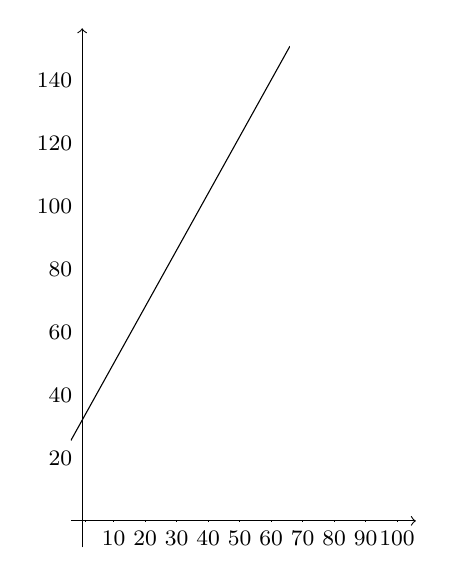
\begin{tikzpicture}[scale = 0.04][line cap=round,line join=round,>=triangle 45,x=1.0cm,y=1.0cm]
\draw[->,color=black] (-3.6,0) -- (105.97,0);
\foreach \x in {,10,20,30,40,50,60,70,80,90,100}
\draw[shift={(\x,0)},color=black] (0pt,2pt) -- (0pt,-2pt) node[below] {\footnotesize $\x$};
\draw[->,color=black] (0,-8.4) -- (0,156.45);
\foreach \y in {20,40,60,80,100,120,140}
\draw[shift={(0,\y)},color=black] (2pt,0pt) -- (-2pt,0pt) node[left] {\footnotesize $\y$};
\clip(-3.6,-8.4) rectangle (65.97,156.45);
\draw [domain=-3.6:65.97] plot(\x,{(--32--1.8*\x)/1});
\end{tikzpicture}
\end{center}
\end{exm}
\begin{exm}{6}
A function can be defined by a table of values, like the following:
\begin{center}
\begin{tabular}{|c|c|}
\hline 
$x$ & $y$ \\ 
\hline 
1 & 1 \\ 
\hline 
5 & 4 \\ 
\hline 
9 & 5 \\ 
\hline 
13 & 17 \\ 
\hline 
\end{tabular} 
\end{center}
Here, we can see that $y$ is a function of $x$, since to each $x$ corresponds one and only one $y$.  The domain is $\{1,5,9,13\}$ and the range is $\{1,4,5,17\}$.  A challenging problem is to come up with an explicit rule for the function.
\end{exm}
Armed with the idea of a function, we can better understand the formalist idea of mathematics and some of its limitations.  If mathematics is just rule-governed operations with symbols, then it looks as though it could be done by a computer without any help from a human being.  In fact, that's exactly what computers do; they perform operations on strings of symbols according to rules.  We input a string of symbols, press "Enter" and out comes another string of symbols.  In short, if formalists are right, mathematics could be done completely by machines, and human mathematicians would be unnecessary.

How would these machines work?  We would write a complicated program to figure out whether a particular string of symbols was a theorem.  Remember, a theorem is the conclusion of a formal proof, the last statement in a chain of logical steps. Our program, called a \emph{theorem-proving program}, would be able to check any string of symbols to determine whether or not it was a theorem. We could call this function T.  Its domain would be the set of all strings of symbols allowed in our symbol system, and its range would be 
\begin{center}
$\{\text{theorem},\text{not theorem}\}$
\end{center}   

For example, if the string of symbols  
\begin{center}
$\sigma\mu\kappa\upsilon\varsigma\Gamma$
\end{center} 
were a theorem in our system, we when we ran our program we would get
\begin{center}
$T(\sigma\mu\kappa\upsilon\varsigma\Gamma)= \text{theorem}$
\end{center} 
Once again, this means that the string '$\sigma\mu\kappa\upsilon\varsigma\Gamma$' can be derived from our basic assumptions by following the rules of inference.

The goal of the formalists was to show that all of mathematics can be represented by system of symbols and rules of inference.  All that was needed, they believed, was to find the right set of symbols and inference rules.  It is a remarkable fact that this goal turns out to be impossible.  In 1931 Kurt G\"{o}del (1906-1978), an Austrian logician, proved, using traditional mathematical methods, that, regardless of how we set up our system, there will always be certain strings of symbols that are neither theorems nor non-theorems in our system, but may recognized as true or false by mathematicians. 

In other words, our function $T$ simply won't work for those strings.  Mathematicians call G\"{o}del's result an \emph{Incompleteness Theorem}, because it shows that there is no way to create a formal system that can determine for any string of symbols it contains whether or not that string is a theorem.  There will always be strings of symbols that are `undecidable' in every formal system.  
G\"{o}del's work showed that mathematics cannot be completely turned over to machines, like computers, because there will always be some strings of symbols whose correctness can only be assessed by human beings.  There is no way to build a machine which we can be sure will be able to prove all true mathematical statements starting from a single set of assumptions.  To G\"{o}del, this result meant that mathematics must be something over and above any kind of symbolism.  This led him to become a Platonist, as we mentioned earlier.  G\"{o}del's basic idea was to show that all theorem-proving programs run into insurmountable problems when faced with statements like, "This statement is false."  This is similar to the difficulty we encountered in our discussion of Russell's Paradox.

\noindent
\textbf{Constructivism}

It looks as though none of the approaches we have so far considered gives an entirely adequate account of the nature of mathematics.  To summarize, we have seen that mathematics cannot be about things that are completely separate from the physical world; it is not purely logical, and it seems to be more than just a collection of symbols.  During the latter half of the twentieth century it became increasingly clear that none of the traditional ideas about mathematics were entirely correct.  Some mathematicians began to suggest that, perhaps, mathematics is a much more complex activity than anyone had imagined.  In fact, it began to look like each of the traditional ideas covered only part of mathematics. 
 
     A number of mathematicians and philosophers in recent years have suggested that to understand mathematics we will need to take its many different aspects into account.  Above all, these mathematicians suggest that mathematics is a human creation. Let us call this point of view \emph{social constructivism}.  Its chief proponents include the Hungarian mathematician Imre Lakatos, the British philosopher Karl Popper, and Paul Ernest, a British educational theorist.  According to these men, our mathematical knowledge does not rest on unshakeable foundations, like a direct awareness of numbers or shapes, as the Platonist and intuitionist  claim.  Neither does it rest upon logic or basic facts about sets.  Instead, constructivists believe that mathematics is a creative product of human activity.  They believe that numbers, geometrical shapes, and mathematical patterns were invented by human beings, originally for the purpose of solving practical problems.  For example, the Egyptians introduced the right triangle to assist them in agriculture and architecture; the Babylonians introduced numerals as aids to counting and record-keeping. 
      
     At first triangles and numerals were only tools, like hammers and saws.  Eventually, however, people began to raise questions about the relationships between the parts of a triangle or about whether or not a particular number was prime.  These questions have correct answers, and those answers do not depend upon anyone's opinion.  Human beings invented numbers, according to constructivists, but they did not invent the \emph{properties}, or basic facts about, numbers.  Once numbers have been invented, they come to have a life of their own, much like words, or laws, or Shakespeare's plays.  Constructivists speak of mathematical problems as "autonomous", meaning that they are not invented by us.  Once mathematical ideas have been invented, certain kinds of questions naturally arise.  These questions lead to investigation, to making educated guesses or conjectures, and to efforts to develop proofs.  Lakatos writes, 
\begin{quote}
          mathematics does not grow through a monotonous increase of the
          number of indubitably established theorems, but through the incessant
          improvement of guesses by speculation and criticism, by the logic of 
          proofs and refutations. \footnote{Qtd. in Hersh, \textit{What is Mathematics, Really?}, p. 211 }
\end{quote}  
          
Mathematical results are consequences of our invention of mathematics, but they are unintended consequences.  In other words, mathematics grows and changes in unpredictable ways as we work at it.  This, of course, is also true of other human activities; as Popper says, we often get more out than we put in. 
 
For example, as an artist works on a painting, the development of the painting affects how he does his work.  He might not realize that he was really painting a self-portrait when he thought she was painting a portrait of someone else.  She  doesn't realize this until she begins actually to put paint on the canvas and sees how things are turning out.  As another, more mathematical, example consider a complex game, like chess.  All the rules of chess are man-made, products of the human mind.  Nevertheless, as you may be aware, there are many principles or main ideas of chess strategy that were not completely understood until the game had been played for thousands of years.  These principles were not deliberately included in the rules; they were unintended consequences.  Einstein once remarked, "My pencil is cleverer than I am."  He meant by this that he often did not see the consequences of his ideas until he put them down on paper and began to work with them.  According to constructivists, the same is true of mathematics:  we do not fully understand mathematical ideas until we begin to work with them.  Thus, on a constructivist view, a proper mathematical education will not have its basis in mastering an established body of mathematical knowledge by rote but, rather, will emphasize the importance of the student's reconstructing the process of mathematical discovery underlying fundamental results.  In working results out for himself, the student is able to participate directly in the act of effectively employing mathematical tools and, perhaps--in extraordinary cases--advancing the development of mathematics itself, if only by criticizing standard assumptions.

The great strength of constructivism lies clearly in the emphasis it places upon the informal, creative, and evolving nature of mathematical thought, aspects that are all but neglected by the approaches considered earlier.  To be sure, constructivists have been quite right to emphasize the informal, creative, and evolutionary nature of mathematical thought.  It is undoubtedly true that classical approaches to mathematical thinking have almost universally been guilty of treating mathematical ideas as though they arrived ready-made in the human mind, whereas it has only been by a lengthy process of trial and error, of conjecture and refutation, that mathematics has reached its present form.  But there is a great difference between describing the process of mathematical discovery and describing the body of knowledge discovered.  If mathematical knowledge is, as constructivists maintain, a product of human convention, it is clearly a most extraordinary product.  It is true that certain social conventions, like language, customs of dress, or even traffic laws may come, in time, to seem to be both universal and necessary, but as American drivers may recognize when traveling in Britain, or French speakers in Germany, these conventions are quite easily given up when the circumstances require it.  

This is not true, however, of mathematical judgements, which seem to hold in all places and times and to admit of no possible alternatives.  It seems to be both certain and necessary that, for example, $7 + 5 = 12$.  There seems to be no question of giving up
our belief in this statement.  It is simply inconceivable, short of confusion, that we should believe that $7 + 5 = 13$.  This inconceivability accounts, in large part, for
the apparent necessity of mathematical truths.
  
Constructivists, as we have seen, are well aware of the special status of mathematical knowledge, and, as indicated above, have generally explained the apparent objectivity and universality of mathematics by holding that the relationships among mathematical ideas are not man-made, although the ideas themselves are.  But this view really is not very different from that of the logicists, namely, the view that mathematics consists of nothing more than drawing logical conclusions from given assumptions.  The assumptions may be man-made ideas, but the process of discovering relations between them is not distinguishable from logic, and we saw earlier that logic does not completely capture the nature of mathematical activity.  Constructivism contains important insights, but it fails as a complete framework for understanding the nature of mathematics. 

\noindent
\textbf{Conclusion: One Discipline, Many Faces}

 During the latter years of his life, the philosopher Ludwig Wittgenstein, one of the most influential thinkers of the twentieth century, became well known for his opposition to the notion that it is, or ought to be, possible to state precise definitions of terms employed in our ordinary experience.  Thus, speaking of the term "game", for example, we might attempt the following definition: "a competive activity aiming at a goal".  But solitaire is a game, and it is not competitive.  Moreover, frisbee is a game, but its "goal" is far from obvious.  In this way, our efforts at definition may come to nought.  Nevertheless, games do indeed share what Wittgenstein called a 'family resemblance' by which we are able to recognize them.  This resemblance may not be easily articulated, and there may well be cases which seem to lie at the periphery (Is surfing a game?), but most competent users of our language would agree about what constitutes a game and what does not (Performing brain surgery is \textbf{not} a game.)  There are good reasons for supposing that mathematics has much the same nature.
 
     We have seen that the most strenuous efforts of mathematicians to define their subject in straightforward terms have not been successful, or, more, correctly, have only been partially successful.  In the last analysis it seems fair to say that each of the principal approaches to the foundations of mathematics has identified one aspect of mathematical thought and constructed an account that places a more or less exclusive emphasis on that aspect.  For example, Platonism derives its plausibility from emphasizing the apparent objectivity, universality, and necessity of mathematical knowledge.  On the other hand, logicism is rooted in the observation that mathematics is the most logically rigorous branch of human knowledge, exhibiting the highest possible degree of structure, coherence, and rationality.  It is this deductive structure that makes mathematics universally applicable to other fields and enables mathematical thinking to be employed in all walks of life.  Mathematics is unique among disciplines in its use of precisely defined terms and symbols.  In no other field of human activity is symbolism employed in such a manner. This, no doubt, accounts for the appeal of formalism to a generation of eminent mathematicians.  Finally, mathematics has much in common with both art and science.  With the arts, mathematics shares a deep sense of aesthetic value; nearly all mathematicians would agree that their subject is beautiful.  Furthermore, like the arts, mathematics is a creative discipline, with new ideas and methods constantly being developed.  Like the sciences, mathematics is in pursuit of truth, and any mathematical conjecture is subject to criticism and revision, much like  a scientific theory.  Like great theoretical ideas in the sciences, mathematical ideas that unify seemingly disparate branches of the discipline represent the supreme intellectual achievement of the mathematician.
     
It seems then, that mathematics has not yet been defined adequately.  Perhaps the search for such a definition is fundamentally misguided, or perhaps an ingenious mind may someday adequately express the nature of mathematics.  Whatever may be the case,  several aspects of mathematics will be  especially important to its growth and development in the 21st century.  Let us discuss each of these in turn.
     
First, although its applications will increase exponentially in the future, mathematics will continue to be an inherently abstract discipline, and its level of abstraction will continue to rise.  The abstract nature of mathematics, though often an obstacle to the layperson, is precisely what gives mathematics its universal power to act as a model for nearly every aspect of reality, from the large-scale structure of space-time to the complex workings of nervous systems to the behavior of the nuclei of atoms.   It is nothing short of amazing that on many occasions discoveries of mathematicians working at problems belonging to "pure" mathematics have become cornerstones of scientific theories and technological advances of the widest significance.  This process began in the seventeenth century with Newton's and Leibniz's work on integral calculus and reached a pinnacle in the application of the abstract geometry of Riemann to Einstein's General Theory of Relativity.  Spectacular examples in recent times include the development of the modern computer from the theoretical ideas of Alan Turing, a British mathematician, as well as the ingenious use of binary numbers to make possible the Information Age.
      
Second,  mathematics will continue to grow, generating new methods, concepts and problems.  Its growth will be twofold.  On the one hand, it will be driven by imperatives deriving exclusively from mathematics itself and the many unsolved problems that continue to attract the best mathematical minds.  While solutions are are clearly desirable, as a by-product of ongoing reseach new questions are almost certain to arise and generate yet more unsolved problems.  In this way, the field of mathematical inquiry enlarges and deepens in scope.
       
Mathematical work will also be stimulated by the drive to master the complexities of both the natural and the human world.  This imperative will come not only, as it has traditionally, from physics, but also, and increasingly, from molecular biology, medicine, economics, and neuroscience.  The advent of ever-greater computing power will make it possible to model in real time (or hyper-real time) such phenomena as information processing in the visual cortex, the pharmacological effects on the body of new medicines, and the behavior of large-scale social and economic systems.  At the outer limit we can imagine mathematical models so powerful they can emulate the human mind, both in its cognitive and affective aspects.  We are pursuing that goal today, and the prospects are good that we will attain it, provided we have the insight and ingenuity.

     In the coming century mathematical thought will be, more than ever before, intimately linked to its embodiment in technology.  To be sure, mathematics has always been a calculational science. Geometry takes its name from surveying the earth, while trigonometry has similar origins; in modern times we have the logarithms of Napier, the calculus of Newton, and Charles Babbage's Analytical Engine.  Every generation of mathematicians has made improvements upon the technological capabilities of its forebears.  But in the present situation things are different.  Today, owing to the integration of advanced technology into the framework of everyday life, mathematicians encounter a world already laden with mathematics.  The digital cameras, tablet computers, smartphones, and wifi networks found everywhere in the developed world are a living embodiment of the collective mathematical genius of many generations.  In mathematics today, the primary tool of creative work (the computer), the vehicle of communication (the Internet), and the principal product (the algorithm or computation) are inherently bound up with a technologically complex world.  Paper and pencil will not disappear from the mathematician's desk, nor will his desire to construct proofs that can meet the highest standards of rigor, but one may safely assume that mathematicians will devote the lion's share of their time and energy in the coming century to making the fullest possible use of technology both to develop mathematics on its own terms and to bring mathematics to bear on real-world problems.
       
Certainly, there is no shortage of problems.  Future generations must develop new sources of energy.  They must work to restore the earth's ecological balance.  Medical researchers must make progress in the fight against AIDS, cancer, and heart disease.  Economists must develop reliable models of economic growth that are both sustainable and supportive of basic human needs.  Educators must develop methods of effective teaching so that every student will be able to participate in a complex global economy.  In the coming century the world leaders will face the dual challenge of empowering the creative energies of humanity while at the same time taking adequate precautions, so that individuals bent on violence cannot convert their ill will into acts of mass destruction merely by pressing a button.
  
These tasks will require great imagination.  They will demand attention to detail and rigorous analysis.  They will depend upon technological innovation.  In short, they are tasks ideally suited to the mathematician of the twenty-first century.  

\newpage

\nnarticleheader{Plato and the Philosophical Value of Geometry}{Mickey Fairorth, Haverford '19}
“Let no one ignorant of geometry enter here.” These words, engraved above the doorway, greeted any Athenian bold enough to venture into Plato’s Academy. As a student of Socrates, Plato is known to the world as one of the essential Greek philosophers and as one of the greatest thinkers ever. Whereas Socrates wrote nothing down, choosing instead to dialogue with others, Plato left society with an extensive body of work. Besides transcribing Socrates’ wisdom for the world to access, Plato established his Academy in 387 B.C. for eager minds to discuss philosophy. As a school of abstract thought, the engraving above the doorway begs us to question why Plato insisted his students know geometry before entering the Academy.

Part of the reason Plato demanded a knowledge of geometry was because he himself contributed to this field and found it integral to understanding the world. In particular, Plato believed that the raw elements of the universe were composed of regular, convex polyhedrons. These objects, known as Platonic Solids, have congruent, regular, polygonal faces with an equal number of faces meeting at every vertex. In simpler terms, each face is a regular shape (equilateral triangle, square…), and each face is identical. Only five solids meet these criteria:

\begin{center}
The tetrahedron: four equilateral triangular faces.\\
The cube: six square faces.\\
The octahedron: eight equilateral triangular faces.\\
The dodecahedron: twelve pentagonal faces.\\
The icosahedron: twenty equilateral triangular faces.\\
\end{center}

\begin{figure}[h]
  \begin{center}
    
\includegraphics[scale=.925]{fairorth_platonic_solids.png}
  \end{center}
\end{figure}

While Plato’s conception that the universe is composed of these solids is certainly flawed, he properly emphasized the importance of geometry in understanding the world around us. Thus, before someone could enter his Academy in search of life’s toughest truths, it was fitting to have a basic understanding of the space in which they lived. 
	
More importantly, however, Plato needed his students to grasp geometry because it demonstrated an ability to think clearly. Geometry is built entirely upon axioms, deductions from axioms, and further deductions from simpler conclusions. Axioms, derived from the Greek word axios which means “worthy,” are fundamental statements that cannot and need not be proven. Euclid, the father of Euclidean Geometry, exemplifies axioms perfectly in providing such definitions as, “the angles of a triangle always add up to 180 degrees.” Also called postulates, these axioms are generally obvious and self-evident. From basic axioms, mathematicians have derived theorems, which combine axioms in a logically sound manner to find more specific and helpful geometric rules. One of the most famous theorems is the Pythagorean Theorem ($a^2 + b^2 = c^2$) which can provide the length of a side of a right triangle given the other two sides’ lengths. Mathematicians can also use proven theorems as starting points for further conclusions. 

While it is true that Plato investigated geometry and found it useful in itself, he desired the principles of thought behind the math more than the math alone; Plato was not looking to assemble an academy of mathematicians to prove spatial theorems but rather a collection of thinkers who could reason from one thought to the next. Despite the differences in subject matter, philosophy is built on the exact same principles as geometry. From axioms, such as “good is to be sought and evil is to be avoided,” philosophers deductively reason to other conclusions. For instance, one might assess that stealing is evil, and since evil is to be avoided, stealing must be avoided as well. While simple, in theory, these logical syllogisms become increasingly complicated and difficult to evaluate as they move further away from the axioms. Hence, it is imperative for a thinker to see clearly how one premise moves to the next and how any conclusion relates back to the principles upon which it is founded. 

At the end of the day, Plato is not known as a mathematician; he is a philosopher. However, as a philosopher, he saw the beauty and value of geometry that is often missed in high-school classrooms. In the real world, it is not essential to know the Side-Angle-Side Theorem. Yet, for anyone who wishes to impact those around them, it is necessary to think clearly, to reason from a principle to a conclusion, and to employ logical deduction. Above Plato’s Academy of philosophy stood the words “Let no one ignorant of geometry enter here.” If someday, by some odd chance, I become a geometry teacher, my students will read these words as they exit each day from class: “Let no one ignorant of philosophy exit here.”\\\\

\begin{figure}[h]
  \begin{center}
    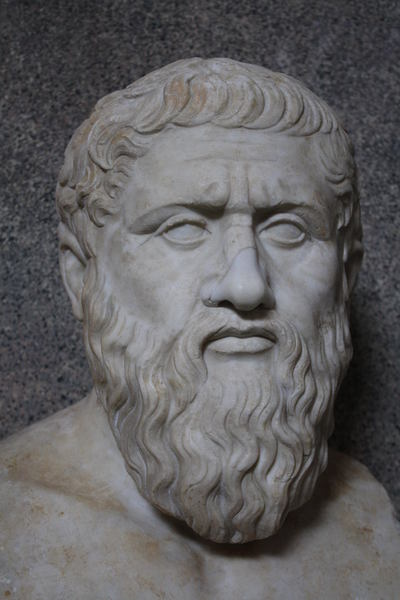
\includegraphics[scale=.8]{fairorth_plato.jpg}
  \end{center}
\end{figure}


\newpage

% Begin the applied math section
\nnwallpaper{2020_Applied_Math_Page_Border.pdf}
\def\currentTitleWallpaper{2020_Applied_Math_Title_Page_Border.pdf}

\addcontentsline{toc}{part}{Applied Mathematics}
\nnimagepage{2020_Applied_Math_Section_Title.pdf}

\definecolor{lightgray}{rgb}{.9,.9,.9}
\definecolor{darkgray}{rgb}{.4,.4,.4}
\definecolor{purple}{rgb}{0.65, 0.12, 0.82}

\lstdefinelanguage{JavaScript}{
  keywords={typeof, new, true, false, catch, function, return, null, catch, switch, var, if, in, while, do, else, case, break},
  keywordstyle=\color{blue}\bfseries,
  ndkeywords={class, export, boolean, throw, implements, import, this},
  ndkeywordstyle=\color{darkgray}\bfseries,
  identifierstyle=\color{black},
  sensitive=false,
  comment=[l]{//},
  morecomment=[s]{/*}{*/},
  commentstyle=\color{purple}\ttfamily,
  stringstyle=\color{red}\ttfamily,
  morestring=[b]',
  morestring=[b]"
}

\lstset{
   language=JavaScript,
   backgroundcolor=\color{lightgray},
   extendedchars=true,
   basicstyle=\footnotesize\ttfamily,
   showstringspaces=false,
   showspaces=false,
   numbers=left,
   numberstyle=\footnotesize,
   numbersep=9pt,
   tabsize=2,
   breaklines=true,
   showtabs=false,
   captionpos=b
}

\hypersetup{
    colorlinks=true,
    linkcolor=blue,
    filecolor=magenta,      
    urlcolor=blue,
}
\urlstyle{same}

\nnarticleheader{A ‘Spin’ on Modeling Propeller Movement}{Kieran Dias-Lalcaca, Elijah Lee, and Ryan Ngo, Haverford '20}
\noindent
\textbf{Introduction}

Propellers have revolutionized the capacity of naval and aeronautical transportation, energy, and dozens of other fields. The idea of being able to propel oneself or some medium through space and time has intrigued us since the Egyptians and Archimedes figured out how to use a screw to lift water out of a river. Thus this technology was revolutionary and is critical to our modern world. At first glance, modeling the operation of a propeller appears to be relatively simple. However, upon closer investigation, one will realize that the behavior of a propeller requires deeper investigation into different axes and dimensions. Using sinusoidal functions, we can model the movement of a propeller as it moves through time. This relationship allows for an inquiry into how sinusoidal functions operate in three dimensions and the relationship between modeling and real-world solutions.

\noindent
\textbf{Breaking it Down}

To start thinking about how we could model a propeller, we decided to break it up into more manageable pieces to figure out the many problems individually. Firstly, we thought of one blade of the propeller rotating on a fixed axis at a fixed forward speed. This limited the number of variables that we had to worry about, but still allowed us to figure out how a system of this complexity would operate mathematically. We decided that GeoGebra was the best way to model this function as Desmos would only allow us to operate in two dimensions. 

With our parameters set and our assumptions noted, we set to work trying to figure out how a sinusoidal function would be used as a model for a propeller. Starting with a general cosine function, as it was decided that it made more sense to start from one extremity or the other rather than in the middle of a rotation, we began to manipulate and play with the different aspects of a sinusoidal function. The amplitude was, somewhat arbitrarily, set as 10 units as the length of the propeller blade should not affect the overall mathematical function. This can be justified due to the fact that because this model for a perfect physics world, without air resistance, torque, or any other of the thousands of other forces that are present in the real world, a purely mathematical model would not change (other than in amplitude, which we want to change). From there we set a period of \(2\pi\), again just as a hypothetical value that would be easy to work with, and then came to the conclusion that all other vertical and phase shifts are negligible. Thus, we had the model of one blade spinning through time and space in one axis, and therefore we could have as many models of propeller blades spinning through time and space in one axis as we wanted by copying our formula. 

This, however, presented the real challenge; despite how many models we wanted to make of one blade spinning through space and time in one axis, we needed to make a model that had multiple blades spinning through space and time in 3 axes. Therefore, we needed to make a system that could model the blades in 3 dimensions. Thus, we arrive at the second stage of thinking in our breakdown of thought, which is the ability to have a 3D model of a blade spinning through space. We eventually came to the idea of a system of functions to define our curve in 3D space.

Within GeoGebra, we made use of the Curve command, which essentially acts as a wrapper for a three function system.
\renewcommand{\thefigure}{1}
\begin{figure}[ht]
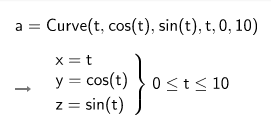
\includegraphics{system.png}
\caption{A screenshot from GeoGebra, showing the breakdown of the Curve command.}
\label{fig:system}
\end{figure}

Looking at Figure 1, we can start to see the structure of the Curve command. The first three parameters define the x, y, and z functions for the curve. Any transformations we want to apply to the curve must be applied to both sinusoidal functions defining the curve. The next parameter specifies the variable, and the last two specify the start and end of the curve (the domain). Using this command, we can easily begin to define our general formula.

This breakdown, described by our general formula, was the result of a lot of trial and error, research with external sources, and much creative thought on how to be able to combine these individual functions effectively.

\noindent
\textbf{General Formula}

Using these realizations, we were able to create a generalized formula/procedure for generating the parameters of the sinusoidal parameters of the curve command in GeoGebra.
For future reference:
\begin{center}
\(\omega\) = angular frequency\\
RPS = rotations per second\\
RPM = rotations per minute\\
\(l\) = number of blades\\
\(t\) = time\\
\(c\) = horizontal shift\\
\(p\) = period
\end{center}

The next step was to determine each of the values which factored into propeller motion. In order to create a model, we used three values: blade length, rotation speed, and number of blades.

We first started with blade length. Because the blades are rotating around an axis, the length is equivalent to the amplitude of any sinusoidal functions. 

Next, we needed to incorporate rotation speed. Rotations are defined in RPMs, or rotations per minute. In our case, one rotation is equivalent to one period. Thus, changing the rotation speed changes the length of one period. In order to use this information, we first have to convert RPMs into RPS (rotations per second). Our time axis is in seconds, so we need our time units to be in seconds as well. 
\[\frac{x\mbox{ rotations}}{1\mbox{ minute}}\cdot\frac{1\mbox{ minute}}{60\mbox{ seconds}}=\frac{x}{60}\mbox{ rotations per second}\]

Next, we can use this information to find the period of our functions. The period is defined as the time for the function to complete one full cycle, or one rotation. We start with rotations per second and we are looking for the time to complete a cycle; in other words, we are looking for seconds (time) per rotations (cycles). The reciprocal of our RPS gives us our period.
\[p=\frac{1}{\mbox{RPS}}\]

Lastly, we have to convert our period into our angular frequency. We can ask: How many times does our function repeat (cycles, or periods) in the same amount of time as the parent function (\(2\pi\))? Here is the equation we can use:
\[\omega=\frac{2\pi}{p}\]

For example, let's say we have a rotation speed of 30 RPMs. First, we start by converting 30 RPM to RPS.
\[\frac{30\mbox{ rotations}}{1\mbox{ minute}}\cdot\frac{1\mbox{ minute}}{60\mbox{ seconds}}=\frac{30}{60}\mbox{ rotations per second}=0.5\mbox{ RPS}\]
Next, we find our period.
\[p=\frac{1}{0.5}=2\]
Finally, we can find our angular frequency. 
\[\omega=\frac{2\pi}{2}=\pi\]

After rotation speed, we needed to factor in the number of blades. This is a little more complex. Depending on the number of blades, the number of curves changes, which requires each curve’s horizontal shift to change. After finding the period of each curve, we can calculate the shift for each curve. 

For explanation, assume a two blade propeller with a period of \(2\pi\). The two curves need to be equally spaced from each other. In other words, the peaks of the second curve needs to land in between the peaks of the first. We can visualize this in Desmos (Figure 2). Shifting the second function by \(\frac{1}{2}\) of the period moves it halfway between the first function’s starting point and the next period. \(\frac{2\pi}{2}=\pi\)

We can modify this reasoning to fit situations with more blades. Generalizing our findings, we can say that the distance between each curve should be \(\frac{p}{l}\). From our previous example:
\[\frac{2\pi}{2\mbox{ blades}}=\pi\]
Another example, keeping our period 2pi but with three blades (Figure 3):
\[\frac{2\pi}{3\mbox{ blades}}=\frac{2}{3}\pi\]
Therefore, the second blade should be shifted \(\frac{2}{3}\pi\) from the first, and the third shifted \(\frac{4}{3}\pi\) from the first (\(\frac{2}{3}\) from the second blade). By multiplying our shift between each blade by the blade number - 1, we get the total shift from the first blade for the given blade. Combining these two findings, we can say that:
\[c_n=\frac{p}{l}\cdot(n - 1)\]
where \(n\) is the 1st, 2nd,...nth blade.
\renewcommand{\thefigure}{2}
\begin{figure}[ht]
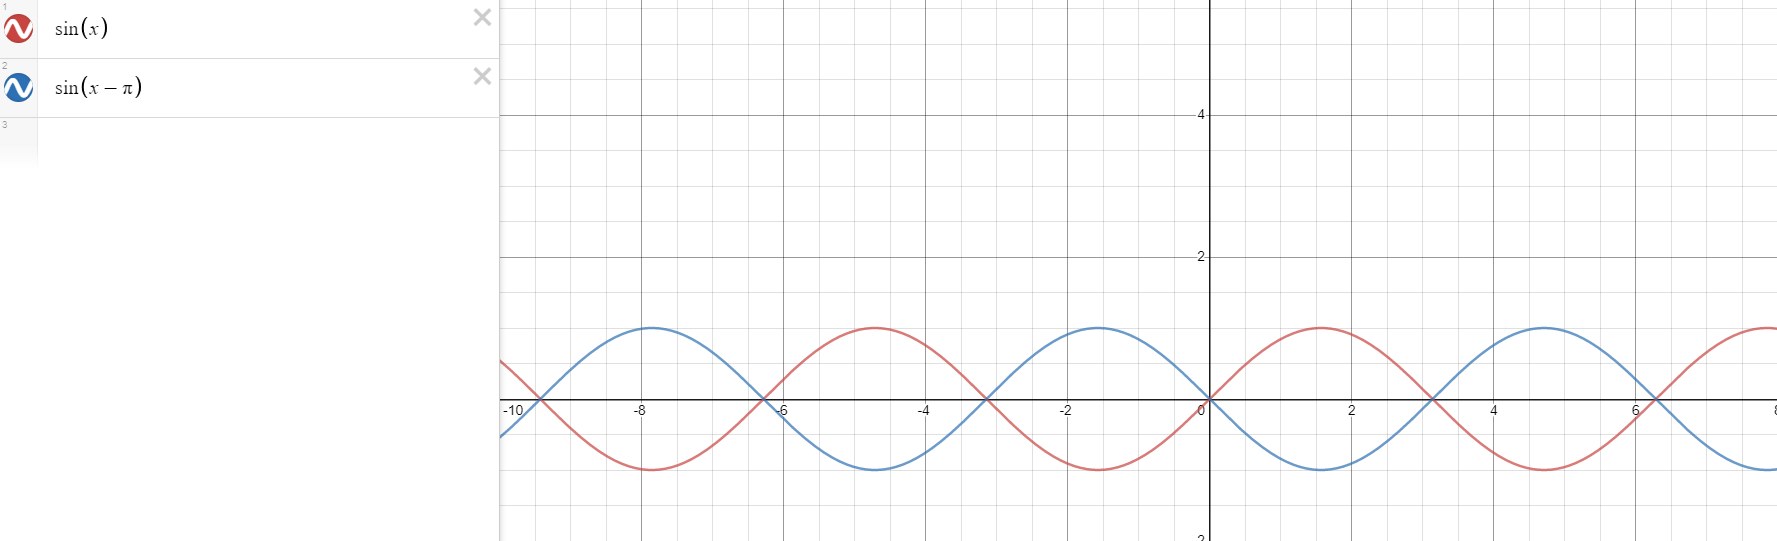
\includegraphics[width=\linewidth]{desmos1.png}
\caption{Desmos graph, showing the proper spacing for two waves}
\label{fig:desmos1}
\end{figure}

\renewcommand{\thefigure}{3}
\begin{figure}[ht]
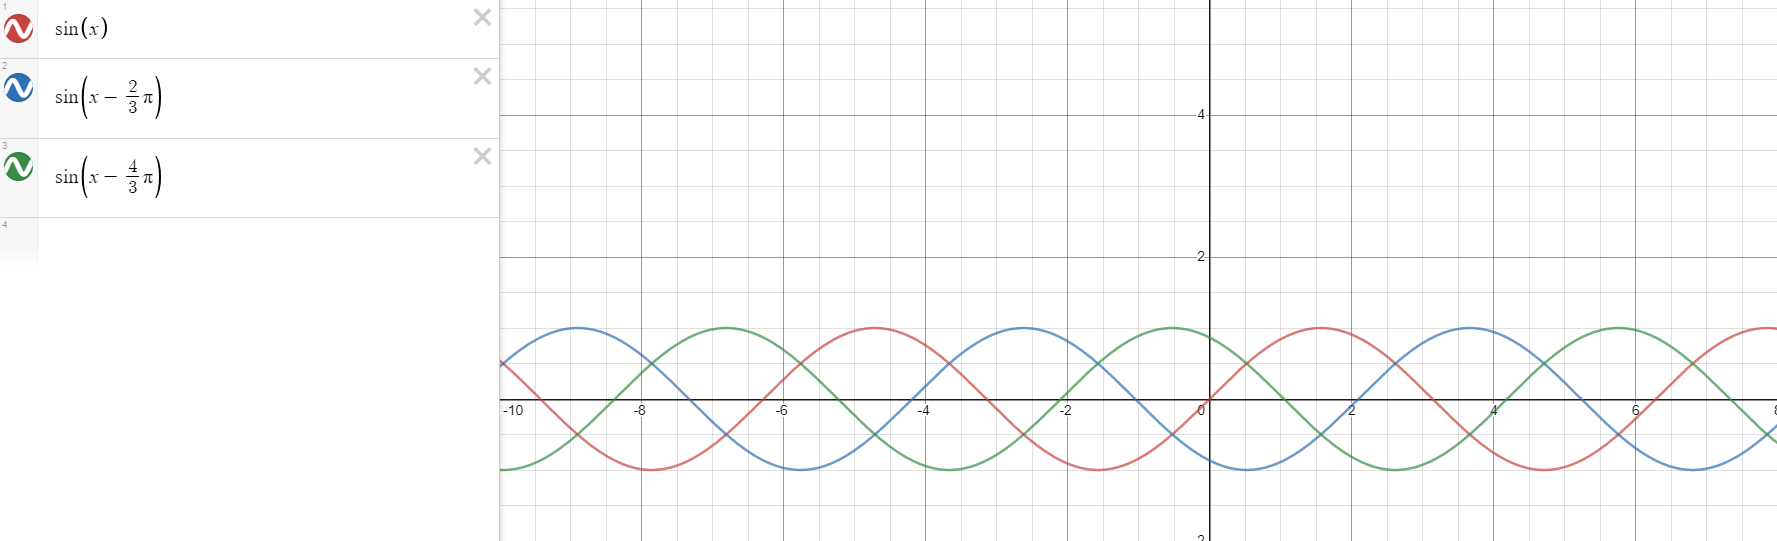
\includegraphics[width=\linewidth]{desmos2.png}
\caption{Desmos graph, showing the proper spacing for three waves}
\label{fig:desmos2}
\end{figure}

Finally, the Curve command requires a start time and end time. Because we are using time as our independent variable, we can start our function at \(t = 0\). The end time is left to the user to define. By leaving the end time up to the user, we can better visualize the movement of the propeller as it moves through time.

Though the equation at first seemed complicated to dive into, after defining each part, it was now only a matter of what type of propeller we wanted to focus on and plugging in values.

\noindent
\textbf{Real-life Application}

In order to use our model to simulate a real-life situation, we found a video of a glass-bottomed boat. \href{https://www.youtube.com/watch?v=EdXxg20XguY}{YouTube Video}

We found a portion of the video where the propeller reached its maximum speed. The video was listed at 30 frames per seconds. By advancing frame-by-frame for thirty frames, we counted two total rotations. The frame rate is 30 FPS; so the propeller had 2 rotations per every thirty frames, or one second. The propeller has three blades (\(l=3\)). 

In order to plot the movement of this propeller, we had to determine its four values. 

First is blade length. While we could not definitively measure the blade diameter from the video due to a lack of scale, this value is not crucial to the other calculations, only affecting the size of the spirals. We chose to leave the blade length as 1. 

Second, we determined the angular frequency from the propeller speed. Using our method from our general formula:
\[\omega=\frac{2\pi}{\frac{1}{RPS}}\Rightarrow\omega=\frac{2\pi}{\frac{1}{2}}\Rightarrow\omega=4\pi\]
\[\therefore p=\frac{2\pi}{4\pi}=\frac{1}{2}\]

Third, we determined the horizontal shift for each curve. According to our formula:
\[c_n=\frac{p}{l}\cdot(n - 1)\]
where \(n\) is the 1st, 2nd,...nth blade.\\
1st blade:
\[c_1=\frac{\frac{1}{2}}{3}\cdot(1-1)=0\]
2nd blade:
\[c_2=\frac{\frac{1}{2}}{3}\cdot(2-1)=\frac{2}{3}\]
3rd blade:
\[c_3=\frac{\frac{1}{2}}{3}\cdot(3-1)=\frac{4}{3}\]

Lastly, we used a slider to represent the end time. By using a slider, we can “scroll” through the simulation and see the propeller locations at any time.

Putting all these arguments together yields three curve functions.
Click this link to see the fully plotted example in GeoGebra. By manipulating the v slider, you can change the end point of the graph.
\url{https://www.geogebra.org/classic/m9z6frdr}

\noindent
\textbf{Going Further}

Using the aforementioned general formula, we wanted to create a fully customizable and parameterized simulation. By utilizing the scripting feature within GeoGebra, we were able to fully integrate the steps needed to generate our functions straight into our GeoGebra project. Figure 4 shows an example use of the capabilities of our simulation.
\renewcommand{\thefigure}{4}
\begin{figure}[ht]
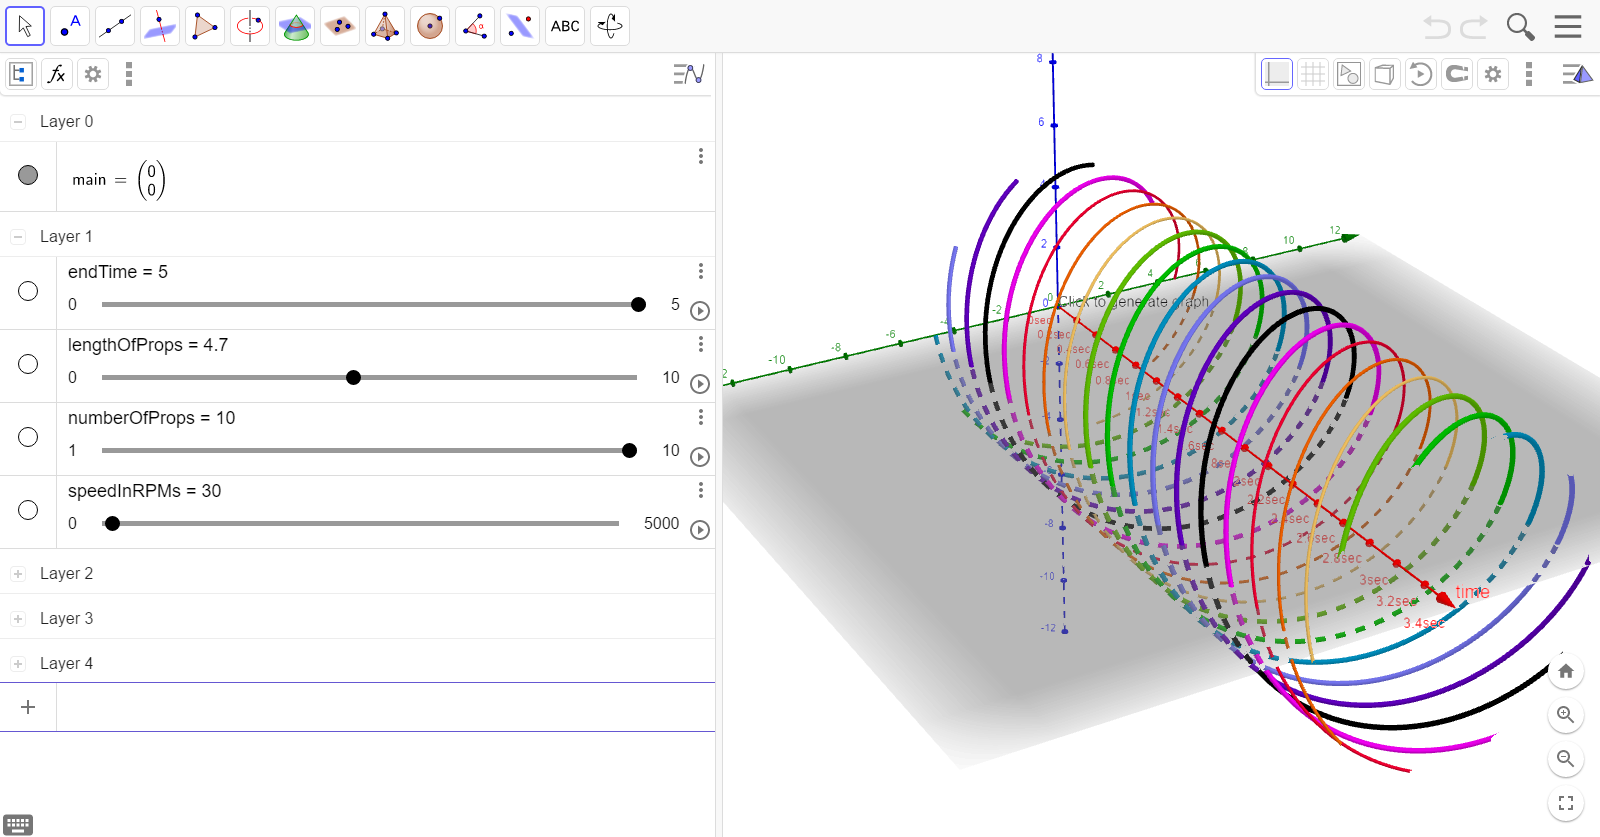
\includegraphics[width=\linewidth]{simuex.png}
\caption{An example simulation.}
\label{fig:simuex1}
\end{figure}

Click this link to access our fully scripted and parameterized simulation: \url{https://www.geogebra.org/classic/y4d4kaua}

\noindent
\textbf{Simulation Explanation}

Layer 0 contains a “main” object, centered at the origin. This object handles the main calculations for the simulation. Each time parameters are edited, clicking on this object recalculates the simulation.
Listing \ref{lst:jscode} shows a cleaned version of the JavaScript behind the main object. This script controls the visibility of objects, angular frequency, and each function's horizontal shift.
\begin{lstlisting}[caption={JavaScript attached to main object},label={lst:jscode},captionpos=b]
// Setup inputs
var numProps = ggbApplet.getValue("numberOfProps");
var speedRPM = ggbApplet.getValue("speedInRPMs");
var amp = ggbApplet.getValue("lengthOfProps");
var end = ggbApplet.getValue("endTime");


// Hide all spiral objects
for (var i = 97; i <= 106; i++) {
    ggbApplet.setVisible(String.fromCharCode(i)+String.fromCharCode(i), false);
}

// Show number needed
for (var i = 97; i <= 97 + (numProps - 1); i++) {
    ggbApplet.setVisible(String.fromCharCode(i)+String.fromCharCode(i), true);
}

// Calculate angular frequency
var rps = speedRPM / 60;
angFreq = (2 * Math.PI) / (1 / rps);
ggbApplet.setValue("ang", angFreq);

// Generate spiral offsets
for (var i = 0; i < numProps; i++) {
    var shiftName = String.fromCharCode(i + 97) + "shift";
    ggbApplet.setValue(shiftName, ((1 / rps) / numProps) * i);
}

\end{lstlisting}

Working through Listing \ref{lst:jscode}:

Lines 1-5 grab values from the input slider and assign them to local variables for later use. Next, the script hides each of the curve functions. Lines 8-10 loops through the letters a-j, and hides the correspondingly named objects. The script then shows the necessary number of objects in a similar fashion (lines 13-16). Lines 18-21 calculates the global angular frequency, and outputs the value back into an object. Lastly, lines 23-27 generate the horizontal shift for each function, following the general formula.

Layer 1 contains all of the parameters. You can use the sliders or directly input desired values into the fields. Each time an edit is made, click on the main point to recalculate the simulation.

Layer 2 holds all of the curve functions. This simulation supports a maximum of ten propellers; thus, there are ten curve functions. GeoGebra scripting does not support the creation of new objects. Therefore, it is easiest to pre-create objects and activate them as needed. To avoid using reserved letters (e, i, etc.), function names are doubled up. Using this function as an example:
\[\mbox{aa}=\mbox{Curve}(t, \mbox{amp}\cdot\cos(\mbox{ang}(t-\mbox{ashift})), \\ \mbox{amp}\cdot\sin(\mbox{ang}(t-\mbox{ashift})), t, 0, \mbox{endTime})\]

We are using the Curve command built in to GeoGebra, as before. The parameters remain identical. However, there are additional elements to the sinusoidal functions.
\[\mbox{amp}\cdot\cos(\mbox{ang}(t-\mbox{ashift}))\]
amp is a variable linked to the propeller length parameter. It represents the amplitude of the sinusoid, and is identical for each curve.

ang represents the angular frequency. It is linked to the propeller speed parameter. Using the same method from the general formula, RPMs are converted into rotations per second, which is then used to calculate the angular frequency. This value is also equivalent for all of the curves.

ashift represents the horizontal shift of the sinusoid. Each curve has a different horizontal shift; the script calculates each shift using the method in the general formula and then sets the appropriate variable in Layer 3 to its corresponding value. Layer 3 contains all of the shift variables. Layer 4 contains the amplitude variable, and the angular velocity variable.

\noindent
\textbf{Summary}

In closing, we found an efficient and concise process to properly model propeller movement. Through the investigation process, we had many realizations about the behavior of sinusoids. In addition, the complexity of modeling a function in three dimensions allowed us to dig deeper not only into sinusoids, but also in defining a function in 3D space. Using GeoGebra allowed us to visualize the changes we made, and see how changes to different parts of our function affected the 3D spiral in different ways. As we investigated, we encountered many different situations which prompted further investigation. Especially when investigating the new three dimensional space, many “side investigations” took place to help explain “why?”. We think that our model is an accurate representation of real-life conditions. However, studies have found that real-life movement deviates from models. As seen in Figure 5, actual propeller movement varies slightly from the modeled theoretical path. Despite this inconsistency, our model still provides an accurate depiction of ideal propeller movement.

\renewcommand{\thefigure}{5}
\begin{figure}[h]
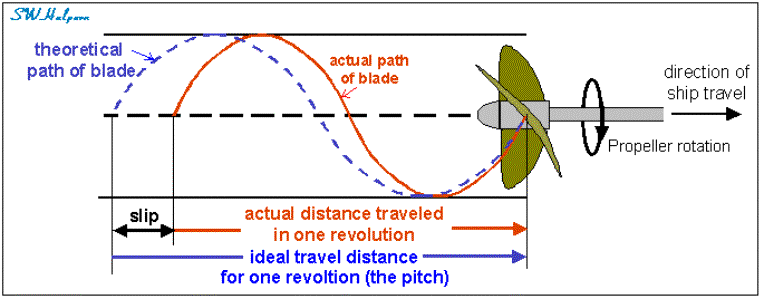
\includegraphics[width=\linewidth]{image019.png}
\caption{Diagram comparing the ideal theorized movement of a propeller vs. actual movement. (Source: www.titanicology.com/)}
\label{fig:real}
\end{figure}

Our goal was to provide the viewer with a simple simulation of propeller movement through time. Through this simple simulation, it is clear that propeller movement is just one of many examples of sinusoids in our world. After all, Da Vinci once said, “Simplicity is the ultimate sophistication.”

\newpage

%\documentclass[10pt,a4paper]{article}
%\usepackage[utf8]{inputenc}
%\usepackage{amsmath}
%\usepackage{amsfonts}
%\usepackage{amssymb}
%\usepackage{graphicx}
%\graphicspath{ {./assets/} }
\nnarticleheader{Lagrange Points: Solving for Gravitational Parking Spaces}{Alexander Greer, Haverford '20}
\textbf{Introduction}
\newline

Picture your middle school science class: you are working through a unit on forces and your teacher is making an analogy for gravity. He has set up a big rubber sheet, at the center of which he has placed a heavy steel ball. The ball weighs down the sheet to form a sort of funnel. He then places a marble at the edge of the sheet and asks you what might happen if he lets go. You, being a well-informed science student, suggest that the marble will roll around and around the funnel created by the ball in a sort of orbit. Your teacher releases the marble and it follows exactly the path you expected. Then, your teacher recovers the small marble, adds another steel ball before asking another question: what will happen to the path of the marble if it conserves its angular velocity given that the entire sheet is in a rotating reference frame?

This, obviously far beyond the scope of a middle school science class, turns out to be a very difficult problem to solve. It is called the \textit{three-body problem} and has challenged physicists and mathematicians since Newton developed his laws of motion. Through centuries of study, we have found that there is, in fact, no closed-form solution to the motion of three bodies. That is, subsequent movement of the bodies cannot be predicted without equations of infinite magnitude.

Applications of the three-body problem are not entirely hopeless, however. Systems like the Earth, Moon, and Sun indicate that there has to be some quantifiable pattern in behavior. One method is to solve a \textit{restricted} three-body problem, defined by one body of negligible mass under the influence of two more massive bodies. In 1772, Franco-Italian mathematician and astronomer Joseph-Louis Lagrange discovered a series of points at which such a body could maintain a stable position relative to the movement of the other two. A small enough object would be caught in a series of opposing gravitational forces that all cancel out. These five “Lagrange Points” are extremely useful for astrophysicists to “park” objects in space. Things like satellites can remain in a stable position without falling into orbit around the two massive bodies while requiring minimal energy to do so.
\newline\newline
\textbf{Explanation}
\newline

Three of these Lagrange points (notated $L_1,$ $L_2,$ and $L_3$) exist collinearly on the axis defined by the two massive bodies. They are “nominally unstable,” meaning they require some energy input in order for a third body to maintain position over long periods of time. The other two points ($L_4$ and $L_5$) are at the corners of equilateral triangles in the plane of orbit whose common base is the line between the centers of the two massive bodies. In the solar system, many natural satellites can be found around the $L_4$ and $L_5$ points of various planets, as they are naturally stable and provide undisturbed equilibrium (Figure 1). 

\begin{figure}[h]
  %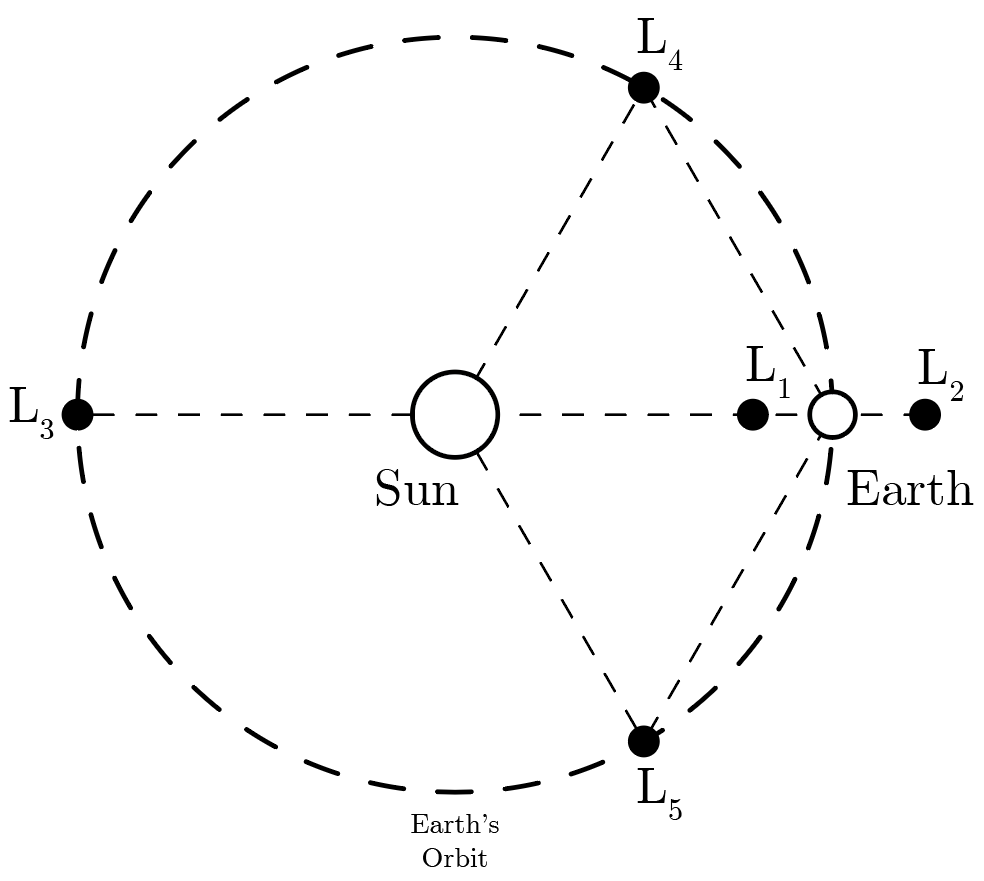
\includegraphics[scale=.5]{greer_lagrange_fig_1}
  \caption{The five Lagrange points.}
  \label{fig:1}
\end{figure}

The derivation for these points is based on Newton’s Law of Gravitation, which describes the force of gravity between two objects based on their masses and distance from one another: \[F_g = G\frac{m_1m_2}{r^2}\]

$m_1$ and $m_2$ are the masses of both objects in kilograms, $r$ is the distance between the two in meters, and $G$ is the gravitational constant equal to $6.674\times{10^{-11}} \frac{m^3}{kg\cdot{}s^2}$.
\newline\newline
\textbf{Derivation}
\newline

Unfortunately, because of the physical nature of our universe, there is no simple law of gravitation for three distinct bodies. That would make this problem a whole lot easier. To find Lagrange points in a restricted three-body problem, we can certainly apply the Law of Gravitation, but we’ll end up approximating the points’ positions. For the use cases on Earth, however, these approximations are more than adequate. 

We can observe the figure below (Figure 2) to see how each of the masses act on each other. 

\begin{figure}[h]
  %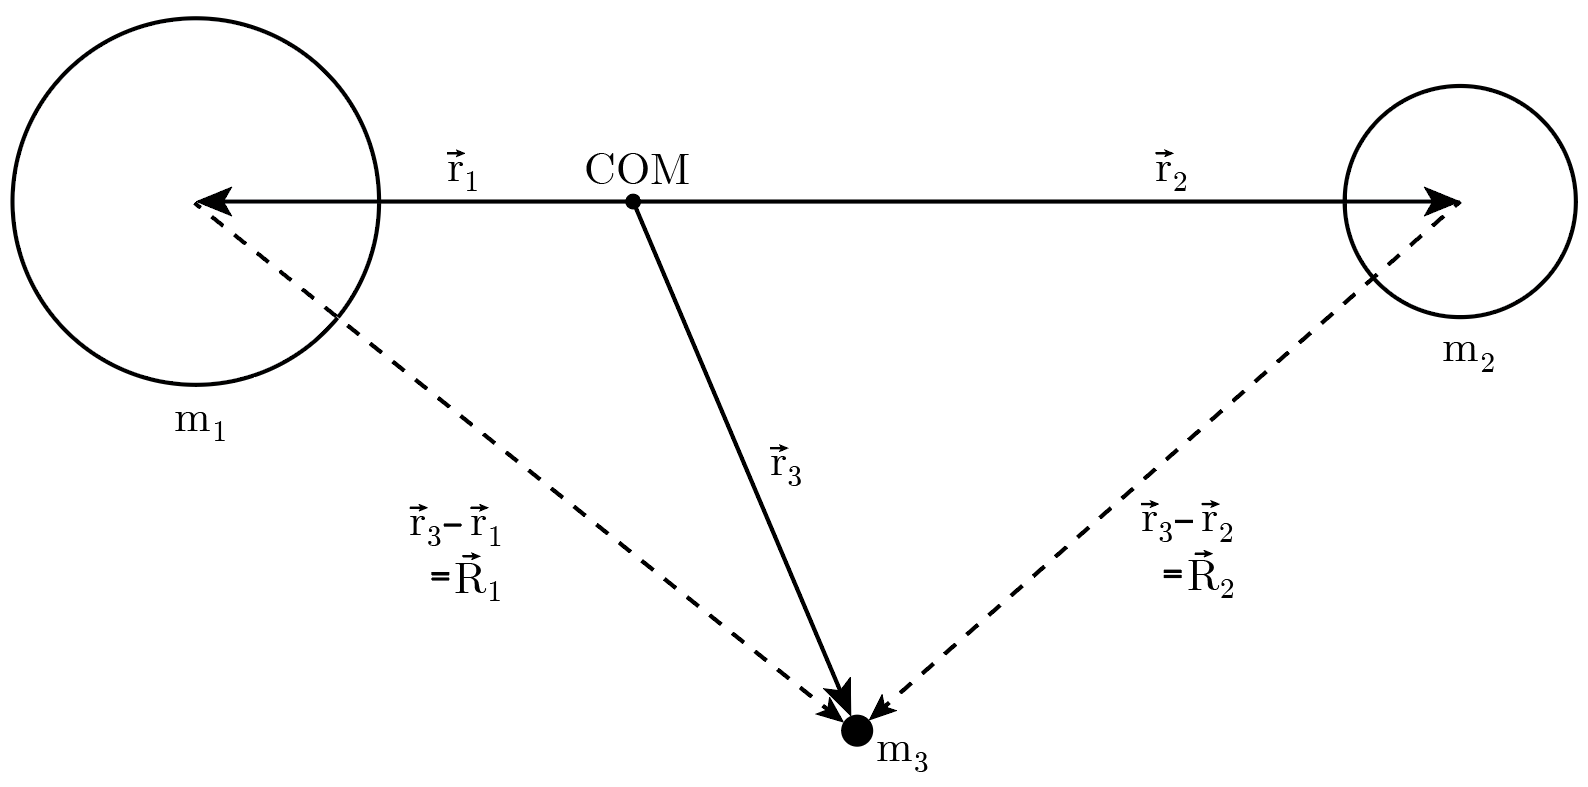
\includegraphics[scale=.5]{greer_lagrange_fig_2}
  \caption{Gravitational forces in a restricted three body problem.}
  \label{fig:2}
\end{figure}

$m_1$ and $m_2$ are the large masses of this system (for example, the Sun and the Earth). $m_3$ is the third mass of negligible magnitude. We use position vector representations of the distances between objects. These are relative to the system’s center of mass (COM). $\vec{r_1}$, $\vec{r_2}$, and $\vec{r_3}$ represent the positions of $m_1$, $m_2$, and $m_3$, respectively. We can denote the direction of the forces acting on m3 by subtracting each other mass’ position vector. The force of $m_1$ on $m_3$ is in the direction of $\vec{r_3}-\vec{r_1}$, which we can denote as $\vec{R_1}$. Thus the force of $m_2$ on $m_3$ follows $\vec{r_2}-\vec{r_1}$, denoted as $\vec{R_2}$

The total force on $m_3$ equals the sum of the forces on it by both $m_1$ and $m_2$, as below: 
\[F_T=F_{1\rightarrow3} + F_{2\rightarrow3}\]

Plugging in our position vectors, we arrive at the below equation:
\[F_T=G\frac{m_1m_3}{|\vec{R_1}|^2}\hat{R_1}+G\frac{m_2m_3}{|\vec{R_2}|^2}\hat{R_2}\]
which can be simplified as:
\[F_T=m_3G(\frac{m_1}{|\vec{R_1}|^2}\hat{R_1}+\frac{m_2}{|\vec{R_2}|^2}\hat{R_2})\]

$\hat{R_1}$ and $\hat{R_2}$ denote unit vectors in the directions of the present forces, equal to $\frac{\vec{r_3}-\vec{r_1}}{|\vec{r_3}-\vec{r_1}|}$ and $\frac{\vec{r_3}-\vec{r_2}}{|\vec{r_3}-\vec{r_2}|}$, or $\frac{\vec{R_1}}{|\vec{R_1}|}$ and $\frac{\vec{R_2}}{|\vec{R_2}|}$, respectively. 
\newline

Another aspect that plays into our derivation is the angular frequency ($\Omega$) of the entire system. In our sun-Earth example, there are pseudo-forces acting on the third mass based on the orbital rotation of the entire system. This is described by Kepler’s Third Law of Planetary Motion:
\[\frac{r^3}{T^2}=\frac{G(m_1+m_2)}{4\pi^2}\]
where $r$ is the radius of the orbit and $T$ is the orbital period. Angular frequency is equal to $\Omega=\frac{v}{r}$, and the orbital period is equal to $T=\frac{2\pi r}{v}$. Knowing this, we can plug in and do some algebraic shuffling to get:
\[\Omega^2r^3=G(m_1+m_2)\]
which can then be used to solve for angular frequency:
\[\Omega=\sqrt{\frac{G(m_1+m_2)}{r^3}}\]

The final piece to our puzzle is to quantify the pseudo-forces acting on our system described previously. A rotating reference frame implies the addition of both the Coriolis force and the centrifugal force. The Coriolis force (known commonly as the Coriolis effect) is responsible for things like cyclone formation as the Earth spins, and you may remember the centrifugal force from your middle school science teacher swinging a bucket of water above their head. 
	We account for these pseudo-forces by subtracting out their values from the force equation derived above:
\[F_{\Omega}=F_T-2m(\Omega\times\frac{dr}{dt})-m\Omega\times(\Omega\times r)\]
where the Coriolis force is $-2m(\Omega\times\frac{dr}{dt})$ and the centrifugal force is $-m\Omega\times(\Omega\times r)$.

Performing a bit more inference using equations involving generalized potential energy (see the sources for an in-depth explanation), we can plot our result using a computer program on a 3D contour map (Figure 3).

\begin{figure}[h]
  %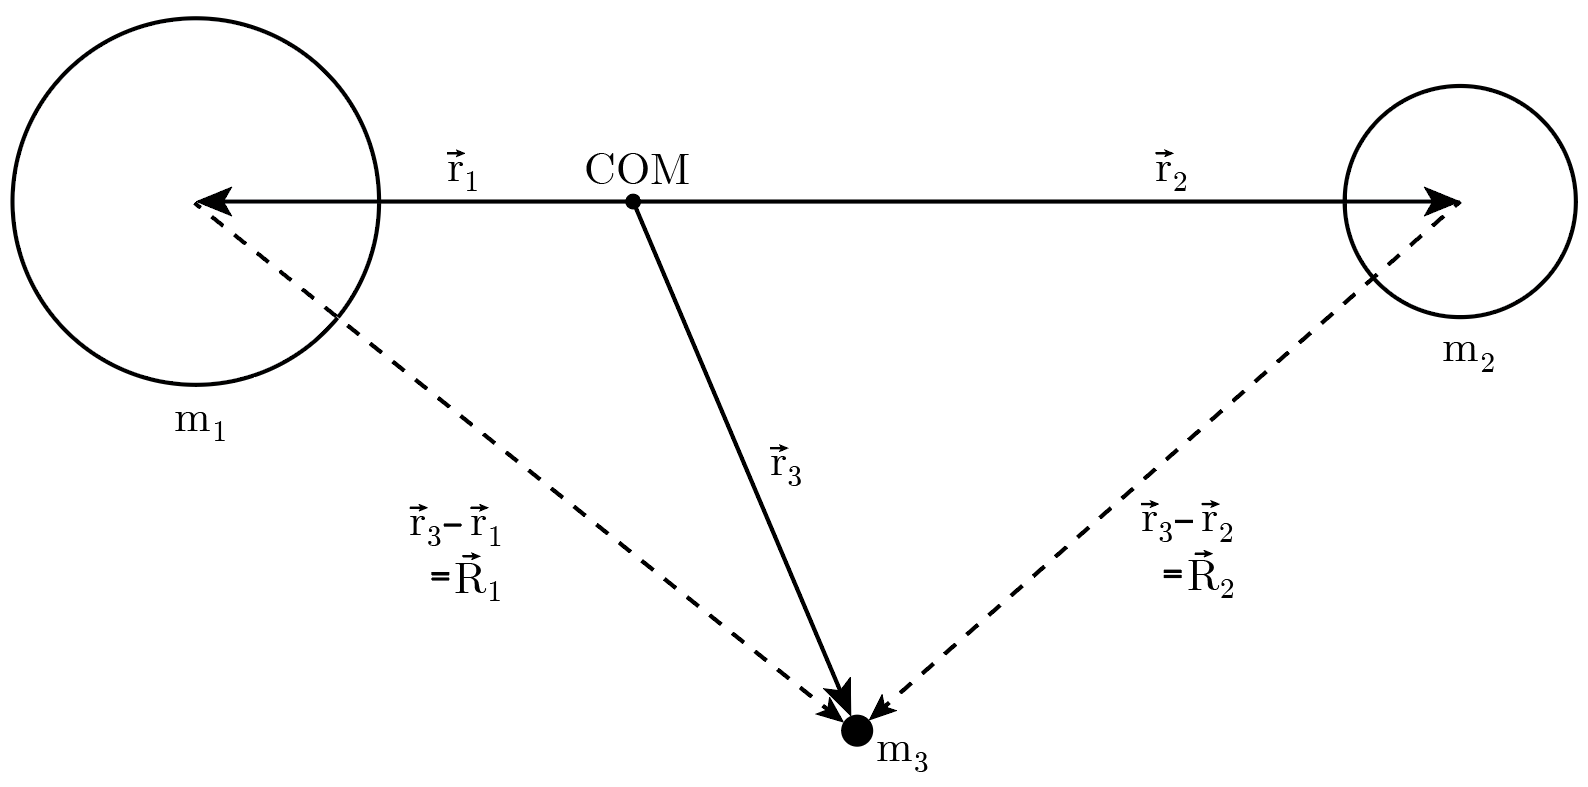
\includegraphics[scale=.5]{greer_lagrange_fig_2}
  \caption{A contour map of gravitational energy revealing the locations of the five Lagrange points.}
  \label{fig:3}
\end{figure}

The extrema of this graph display places where the various gravitational potentials cancel out: the Lagrange points. In the sun-Earth system, points $L_1$ and $L_2$ are about 1.5 million kilometers on either side of the Earth. $L_3$ is approximately opposite Earth at its orbital distance of about 150 million kilometers. $L_4$ and $L_5$ are each 1.5 million kilometers away from Earth at 60-degree angles.
\newline\newline
\textbf{Conclusion}
\newline

The math to get here may have been a bit complicated, and there were certainly some aspects left out for clarity, but at its essence, this derivation demonstrates the simplistic beauty of the laws of our universe. Something as simple as two objects floating around each other can produce complex curves and dips in spacetime where asteroids, satellites, and telescopes can float without worry. Maybe one day in the future humanity will escape the bonds of Earth and rest comfortably in a gravitational valley created by its home planet, looking out at the unknown wonders hidden amongst the stars. 

\newpage

\input{articles/obuz-path-generation.tex}

\newpage

\nnarticleheader{Team $\#$14169 M3 Challenge Submission: Keep on Trucking}{Alexander Greer '20, Gary Gao '21, and Xiaolong Huang '21}

\begin{center}
\textit{This article is an excerpt from Haverford's submission to the 2020 MathWorks Math Modeling (M3) Challenge. Teams of students were tasked with finding mathematical solutions to a large-scale problem over the course of 14 hours. If you are a rising junior or senior interested in participating in next year's competition, contact Mr. Bridge.}
\end{center}

\noindent
\textbf{Executive Summary}

Humanity’s ever-increasing reliance on technology necessitates a strong focus on environmental conservation and clean energy to ensure a safe and prosperous future. One goal of this effort is the use of electric vehicles in place of typical fossil fuel-based transportation. Diesel-powered semi-trucks account for a uniform 12\% of the transportation market, and so replacing these vehicles with electric counterparts would be an effective first step in the transition to wholly-electric transportation.

Here we present the answers to several logistical questions in the effort of switching the diesel semi-truck industry over to electric vehicles. One question is to determine how many electric semis will take over the trucking industry in the future. This is a question of when rather than if. Here, we make an informed prediction of this value based on data related to the current rate of production of semi-trucks throughout the country.

Another question is how to best position charging stations for electric semis along common trucking routes (or “corridors”). The optimal positioning of such stations is influenced by factors such as vehicle range and traffic flow. Here we present optimized charging locations along five standard corridors based on route length, battery capacity, and traffic information throughout each road.

A final question is to determine the prioritization of the development of the above electric stations. While electric vehicles will provide long-term benefits to our society, there may be short term consequences that result from infrastructure changes. Here we outline a prioritization order for the same five routes based on multiple economic and social factors such as political and economic support, as well as route length and associated traffic volume.

The conclusions outlined above and described more thoroughly throughout this work serve to incite the development of electric vehicle implementation. We hope that a broader understanding of the factors at play will lead to widespread adoption and the eventual universal acceptance of environmentally-conscious technologies.

\noindent
\textbf{Definitions}
\begin{itemize}
\item \noindent Commercial Battery Electric Vehicle (\textbf{CBEV} or \textbf{BEV})\\
\indent The above acronym will be used interchangeably to refer to electric semis.

\item \noindent Short Haul (\textbf{SH}), Regional Haul (\textbf{RH}), and Long Haul (\textbf{LH})\\
\indent The abbreviated forms of these vehicle types will be used for the sake of brevity.
\end{itemize}

\noindent
\textbf{Restatement of Problem \#2: "In It for the Long Haul"}

In this problem, we intend to determine the number of necessary CBEV charging stations for each of the five routes provided by the problem (San Antonio, TX to New Orleans, LA; Minneapolis, MN to Chicago, IL; Boston, MA to Harrisburg, PA; Jacksonville, FL to Washington, DC; Los Angeles, CA to San Francisco, CA). Additionally, we will determine the quantity of individual chargers necessary at each station. 

\noindent
\textbf{Assumptions}

\begin{assumption}
Multiple routes can be taken between two cities. Here we assume that drivers will always take the shortest route.

Justification – Drivers always seek to optimize their driven performance, which primarily involves fuel/energy efficiency. Therefore, we assume drivers will select the shortest route in order to expend the least amount of fuel/energy.
\end{assumption}

\begin{assumption}
Secondly, we assume that the drivers will have an 80\% charged battery at the start of their trip, and the driver will try to charge their truck whenever the battery is below 20\%.

Justification – Battery is optimally charged from 20 to 80 percent. The drivers and corporations will seek efficiency to maximize profit, so they will always charge their batteries in this way.
\end{assumption}

\begin{assumption}
Thirdly, we assume that there are a sufficient amount of charging stations around the city, and the charging stations on the highway are left to be built.

Justification – Cities are far more developed than highway resting stops and negates the need for developing new charging stations. In contrast, highway resting stops are spread far apart and are less incentivized.
\end{assumption}

\begin{assumption}
We assume that the traffic flow for semi trucks is constant throughout the day.

Justification – There is a large enough quantity of traffic flowing through the specified routes in order to assume a constant flow.
\end{assumption}

\begin{assumption}
Additionally, we assume that a CBEV battery has a 550 kWh capacity, and the distance to travel when fully charged is 250 miles.

Justification – These numbers fall within the average range and were the most common we found online, thus we used them in our calculations.
\end{assumption}

\noindent
\textbf{Data}
\begin{center}
	\begin{tabular}{|c|c|c|}
		\hline
		\textbf{Truck} & \textbf{Battery Size} & \textbf{Distance to Travel}\\
		\hline
		Freightliner eCascadia & 550 kWh & 250 miles\\
		\hline
		Chanje V8100 & 150 kWh & 150 miles\\
		\hline
		Tesla Semi Truck & Approximately 600 kWh & 300 miles\\
		\hline
	\end{tabular}
\end{center}
\medskip
\begin{center}
	\begin{tabular}{|c|c|}
		\hline \textbf{Routes} & \textbf{Distance}\\
		\hline San Antonio, TX to/from New Orleans, LA & 543 miles\\
		\hline Minneapolis, MN to/from Chicago, IL & 408 miles\\
		\hline Boston, MA to/from Harrisburg, PA & 390 miles\\
		\hline Jacksonville, FL to/from Washington, DC & 706 miles\\
		\hline Los Angeles, CA to/from San Francisco, CA & 382 miles\\
		\hline
	\end{tabular}
\end{center}

\renewcommand{\thefigure}{1}
\begin{figure}[h]
  \begin{center}
    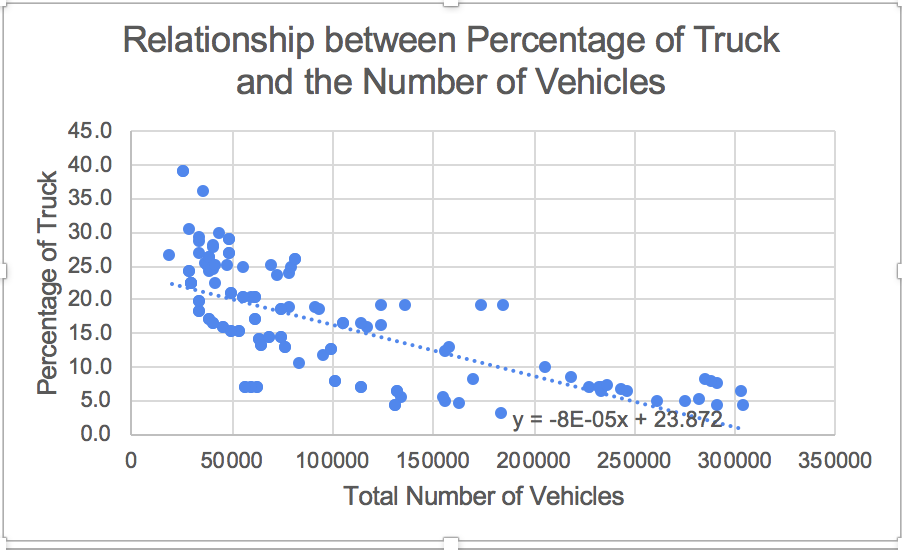
\includegraphics[scale=.95]{M3_image}
  \end{center}
  \caption{Corridor Data, MathWorks Math Modeling Challenge 2020, https://m3challenge.siam.org/node/478}
  \label{fig:1}
\end{figure}

\noindent
\textbf{Analysis}

We define distance to be D miles, charging speed to be C kW, battery size to be B kWh, distance that a truck can drive to be K miles, Price of each charger to be P dollars, average amount of semi trucks that passes through a certain point every day to be A trucks/day, the number of charging stations to be R, and the number of chargers at each station to be S.

We first look at the average amount of class 8 trucks here. From Corridor Data, MathWorks Math Modeling Challenge 2020, url, we can obtain the amount of total vehicles at a certain and the number of trucks at the certain point of the given route. However, the data of numbers of trucks are missing at certain points of the table. In order to obtain the missing data, we can take the average of the ratio between the number of trucks and the number of total vehicles to approximate the number of trucks when given the number of total vehicles.

We define the number of trucks to be B. We notice that the number of trucks is not equivalent to the number of class 8 trucks, so we can approximate the number of class 8 trucks by comparing the total number of trucks to the total number of semi trucks. We know that the number of semi trucks is 2 million and the total number of trucks is 15.5 million. Hence, we can approximate the number of semi trucks at a given point on the highway by: 
\[A = \frac{2}{15.5}\cdot B\]
\indent However, if we look at the graph of all available traffic data of percentages of Truck and total number of vehicles, we can see that the percentage of trucks when there are fewer vehicles is significantly higher than that when there are more vehicles, which suggests that the number of trucks tend to remain the same. Hence, we apply a linear regression on this set of data and add that function to our model. We define the number of vehicles to be E, which is as below:
\[A = \frac{2}{15.5}\cdot B = \frac{2}{15.5}\cdot(-8\cdot10^{-5}\cdot E+23.872)\cdot E\]
\indent We now have the number of trucks at a certain location. We then try to determine how many stations are needed for a route. Considering the cost, we will try to find the minimum charging stations that can fulfill the need. We know that, optimally, the truck is going to use 60\% of its battery, which is derived from our assumption that the truck is going to start at 80\% battery and charge whenever the battery gets below 20\%. Hence, we have the model: 
\[R = \frac{D}{\displaystyle \frac{3}{5}\cdot K}\]
\indent We now obtain models that can calculate the number of stations for a given route, and now we need to find out how many chargers are necessary for each station. We first need to determine how long it takes for a truck to charge. The time, which is defined as T, is equal to 60\% of the battery size (since we are only charging from 20\% to 80\%) divided by the charging speed, which is:
\[T = \frac{3B}{5C}\]
\indent We know that there are 24 hours in a day, and the number of trucks is the truck that passes through the place in that 24 hours. We also know from the last consumption that the traffic flow is constant. Hence, we have:
\[S = \frac{T}{24}\cdot A\]
\indent Now we have the general functions and we need to calculate the number of stations and the number of chargers at each station for each route. 

\noindent
\textbf{San Antonio, TX to/from New Orleans, LA:}

We try to find the number of stations by inserting the equation $\displaystyle R = \frac{D}{\frac{3}{5}\cdot K}$. We know that $D = 543$ miles, $K = 250$ miles. Inserting the constant, we have:
\[R = \frac{550}{150} \approx 4\]

We then try to find the number of chargers at each station:
\begin{align*}
	S &= \frac{T}{24}\cdot A\\
	&= \frac{T}{24}\cdot \frac{2}{15.5}\cdot(-8\cdot10^{-5}\cdot E+23.872)\cdot \frac{E}{100}\\
	&= \frac{1.33}{24}\cdot \frac{2}{15.5}\cdot(-8\cdot10^{-5}\cdot 77580+23.872)\cdot \frac{77580}{100}\\
	&\approx 108
\end{align*}
T
herefore, for each charging station we need 108 chargers. 

\noindent
\textbf{Minneapolis, MN to/from Chicago, IL:}

Similarly, we have
\[R = \frac{408}{150} \approx 3\]

Then,
\begin{align*}
	S &= \frac{T}{24}\cdot \frac{2}{15.5}\cdot(-8\cdot10^{-5}\cdot E+23.872)\cdot \frac{E}{100}\\
	&= \frac{1.33}{24}\cdot \frac{2}{15.5}\cdot(-8\cdot10^{-5}\cdot 103062+23.872)\cdot \frac{103062}{100}\\
	&\approx 115
\end{align*}

Therefore, we need 3 charging stations and for each charging station we need 115 chargers. 

\noindent
\textbf{Boston, MA to/from Harrisburg, PA:}

Similarly, we have
\[R = \frac{390}{150} \approx 3\]

Then,
\begin{align*}
	S &= \frac{T}{24}\cdot \frac{2}{15.5}\cdot(-8\cdot10^{-5}\cdot E+23.872)\cdot \frac{E}{100}\\
	&= \frac{1.33}{24}\cdot \frac{2}{15.5}\cdot(-8\cdot10^{-5}\cdot 75435+23.872)\cdot \frac{75435}{100}\\
	&\approx 96
\end{align*}

Therefore, we need 3 charging stations and for each charging station we need 96 chargers.

\noindent
\textbf{Jacksonville, FL to/from Washington, DC:}

Similarly, we have
\[R = \frac{709}{150} \approx 5\]

Then,
\begin{align*}
	S &= \frac{T}{24}\cdot \frac{2}{15.5}\cdot(-8\cdot10^{-5}\cdot E+23.872)\cdot \frac{E}{100}\\
	&= \frac{1.33}{24}\cdot \frac{2}{15.5}\cdot(-8\cdot10^{-5}\cdot 83803+23.872)\cdot \frac{83803}{100}\\
	&\approx 103
\end{align*}

Therefore, we need 5 charging stations and for each charging station we need 103 chargers.

\noindent
\textbf{Los Angeles, CA to/from San Francisco, CA:}

Similarly, we have
\[R = \frac{382}{150} \approx 3\]

Then,
\begin{align*}
	S &= \frac{T}{24}\cdot \frac{2}{15.5}\cdot(-8\cdot10^{-5}\cdot E+23.872)\cdot \frac{E}{100}\\
	&= \frac{1.33}{24}\cdot \frac{2}{15.5}\cdot(-8\cdot10^{-5}\cdot 134347+23.872)\cdot \frac{134347}{100}\\
	&\approx 126
\end{align*}

Therefore, we need 3 charging stations and for each charging station we need 126 chargers.

\noindent
\textbf{Conclusion}

Now we have tested all the routes and obtained valid solutions. Below is a list of the number of chargers necessary to supply each of the routes provided. 

\begin{center}
	\begin{tabular}{|c|c|}
		\hline \textbf{Routes} & \textbf{Number of Chargers}\\
		\hline San Antonio, TX to/from New Orleans, LA & 108 chargers\\
		\hline Minneapolis, MN to/from Chicago, IL & 115 chargers\\
		\hline Boston, MA to/from Harrisburg, PA & 96 chargers\\
		\hline Jacksonville, FL to/from Washington, DC & 103 chargers\\
		\hline Los Angeles, CA to/from San Francisco, CA & 126 chargers\\
		\hline
	\end{tabular}
\end{center}

\vspace{1.25cm}

\begin{center}
\textit{For more information on\\
the MathWorks Math Modeling Challenge,\\
including winning entries from\\
this year's competition,\\
visit https://m3challenge.siam.org/}
\end{center}


\newpage

% Begin the applied science section
\nnwallpaper{2020_Applied_Science_Page_Border.pdf}
\def\currentTitleWallpaper{2020_Applied_Science_Title_Page_Border.pdf}

\addcontentsline{toc}{part}{Applied Science}
\nnimagepage{2020_Applied_Science_Section_Title.pdf}

\nnarticleheader{tDCS and rTMS: Promising Treatments for Alzheimer’s}{Carson DeMarco, Haverford '20}
What disease currently stands as the sixth leading cause of death in the United States, yet has no cure? Alzheimer’s Disease (AD). By the year 2050, 5.8 million Americans are projected to be diagnosed with AD. Additionally, AD is a heavy financial burden and will cost the United States 290 billion dollars for continued treatment by 2050 \cite{Association}. AD, which primarily affects memory, is a harmful neurodegenerative disease, an irreversible condition leading to gradual degeneration or death of nerve cells in the central nervous system (CNS) \cite{JNPD}. The CNS, which integrates and processes information from the sensory division of the peripheral nervous system, is vital for the human body to function normally, and the malfunction of this system lead to detrimental health issues. While AD remains incurable, two current treatments have proven to enhance cognitive thinking and memory: Transcranial Direct Current Stimulation and Repetitive Transcranial Magnetic Stimulation.

AD disrupts the communication between neurons and kills them. AD first targets and destroys neurons in the brain associated with memory, such as those found in the cerebral cortex (the brain’s memory center) and the entorhinal cortex (the network in the brain for memory, perception of time, and navigation). Additionally, AD targets the hippocampus, the brain region that turns short-term memories into long-term memories. In later stages, AD affects more regions in the cerebral cortex, such as the prefrontal cortex, the center for cognitive thinking and decision making. Symptoms of these later stages include the inability to perform normal daily tasks, such as driving, reading, and communicating. In the final stages of AD, known as brain atrophy, the brain loses volume: enough neurodegeneration has occurred to an extent that the brain actually shrinks in size \cite{Health}.

The emergence of AD is caused by two main issues: Beta-Amyloid Plaques and Neurofibrillary Tangles. Beta-Amyloid Plaques arise by the accumulation of a malformed protein called Amyloid-Beta Precursor Protein (APP) in the cerebrospinal fluid. APP is a transmembrane protein vital for neural growth and repair. A small peptide from this protein can branch-off and leave the membrane, where it changes shape and aggregates into larger molecules, causing plaque formation near the cells \cite{Goodsell}. The Neurofibrillary Tangles emerge from an abnormal version of a protein called Tau. This protein helps to form microtubules, structures that facilitate the transportation of nutrients and essential molecules to different parts in the cell. Abnormal versions of this protein arise when misfolding occurs during protein expression, and a “loose end” sticks out, recruiting more abnormal Tau proteins to attach, leading to the formation of tangles inside the cells. Consequently, the tangles inhibit the neuron from performing normal intracellular functions \cite{Foundation}. Between the two primary factors that lead to AD, the neurons lose their ability to communicate; their dendrites, extensions from the cell that transfer signals, retract and neural connections are lost, leading to neurodegeneration, eventual cell death, and brain shrinkage \cite{Health}. Transcranial Direct Current Stimulation, however, has demonstrated the ability to improve these connections and alleviate the experienced symptoms of AD.

\renewcommand{\thefigure}{1}
\begin{wrapfigure}{R}{0.5\textwidth}
  \begin{center}
    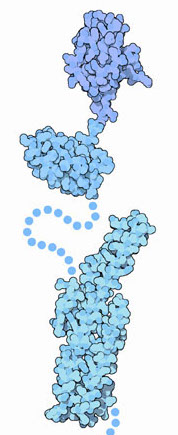
\includegraphics[width=0.26\textwidth]{demarco_app}
  \end{center}
  \caption{A molecular representation of APP}
\end{wrapfigure}

Transcranial Direct Current Stimulation (tDCS) serves as a non-invasive brain stimulation technique shown to improve cognitive abilities and memory associations for individuals affected by Alzheimer’s. tDCS modulates the excitability of a specific brain region by changing the membrane potential, the difference in charge between the inside of a neuron (negatively charged) and the outside of a neuron (positively charged), and modifies the brain circuitries. tDCS has become more prevalent for Alzheimer’s treatment since it promotes neuromodulation, the regulation of controlling neurotransmitters, and cortical changes, improved cognitive functioning. tDCS sends an electrical current across specific brain regions by placing two electrodes on the scalp of the head and has demonstrated improvement in cognitive ability for patients in conducted studies \cite{Machado}.

One study used tDCS for patients with AD to improve their ability to associate pictures with their names. Over the course of ten sessions with 30 minutes of anodal tDCS, a type of tDCS stimulation that excites neural activity, applied to the parietal lobe. The parietal lobe includes brain regions associated with reception and correlation of sensory information. The patients were trained to associate pictures with their corresponding names to show improvements in their cognitive thinking and memory. Several evaluations were conducted: before stimulation, after stimulation, two weeks post-stimulation, and two months post-stimulation. Analysis of the evaluations indicated significant improvements in the patient’s abilities to associate a picture by its name after tDCS. Additional analysis of the parietal lobe after stimulation showed continued improvement beyond the two months post-stimulation evaluation. Thus, tDCS has demonstrated promise to potentially reverse the effects of AD \cite{Chertkow}.

Similarly to tDCS, Repetitive Transcranial Magnetic Stimulation (rTMS) is a non-invasive brain stimulation technique that induces electrical currents based on the principle of electromagnetic induction, the production of an electromotive force across an electrical conductor in a changing magnetic field. The magnetic field is generated by a strong current  circulating within a coiled position in the brain, creating an electrical current through the cortical tissue underneath the coil, delivering rhythmic and repetitive pulses to modulate neural activity. High-frequency rTMS stimulates neural activity, and observations have indicated this stimulation produces positive effects in the brain, such as inducing Long-Term Potentiation (LTP), the consistent strengthening of neural synapses. Several recent clinical trials were conducted to determine the efficacy and safety of rTMS for patients with AD, and the trials presented positive outcomes in cognitive functioning \cite{Dong}.

Alzheimer’s Disease is a deadly neurodegenerative disease. Current promising treatments include the Transcranial Direct Current Stimulation and Repetitive Transcranial Magnetic Stimulation, both non-invasive brain stimulation techniques that are effective for enhancing cognitive function and memory associations damaged by AD. Further and future research into Alzheimer’s should be focused on finding ways to clear and remove the Beta-Amyloid Plaques and Neurofibrillary Tangles in the CNS, not only restoring the health of the affected neurons, but also the health of individuals impacted by the disease.

\newpage
\noindent
\textbf{References}
\begingroup
\renewcommand{\section}[2]{}% https://tex.stackexchange.com/questions/22645/hiding-the-title-of-the-bibliography
%\renewcommand{\chapter}[2]{}% for other classes
\begin{thebibliography}{9}
\bibitem{Alzheimer's}
Alzheimer's, U. A. (2019). The Alzheimer's Crisis. Retrieved January 13, 2020, from
\url{https://www.usagainstalzheimers.org/learn/alzheimers-crisis?gclid=EAIaIQobChMInNS
zrHr5gIVBqSzCh3ykgOpEAAYBCAAEgInD_D_BwE}.

\bibitem{Association}
Association, A. (n.d.). Facts and Figures. Retrieved January 15, 2020, from
\url{https://www.alz.org/alzheimers-dementia/facts-figures}.

\bibitem{Chertkow}
Chertkow, H., Roncero, C., Kneifel, H., Thiel, A., Probst, S., Malus, M., and Solomon, S. (2017,
April 18). Transcranial direct current stimulation (tDCS) improves picture naming in
Alzheimer's Disease and Frontotemporal dementia. (P3.089). \textit{Neurology}. Retrieved January 15, 2020, from \url{https://n.neurology.org/content/88/16_Supplement/P3.089}.

\bibitem{Dong}
Dong, X., Yan, L., Huang, L., \textit{et al}. (2018, October 12).
Repetitive transcranial magnetic stimulation for the treatment of Alzheimer's disease: A
systematic review and meta-analysis of randomized controlled trials. \textit{PLOS}. Retrieved January
15, 2020, from \url{https://journals.plos.org/plosone/article?id=10.1371/journal.pone.0205704}.

\bibitem{Foundation}
Foundation, B. F. (2019, December 11). Amyloid Plaques and Neurofibrillary Tangles. Retrieved
January 14, 2020, from \url{https://www.brightfocus.org/alzheimers-disease/infographic/amyloid-plaques-and-neurofibrillary-tangles}.

\bibitem{Goodsell}
Goodsell, D. (2006, July). PDB101: Molecule of the Month: Amyloid-beta Precursor Protein.
Retrieved January 14, 2020, from \url{https://pdb101.rcsb.org/motm/79}.

\bibitem{Health}
Health, N. I. of. (n.d.). What Happens to the Brain in Alzheimer's Disease? National Institute on
Aging. Retrieved January 13, 2020, from \url{https://www.nia.nih.gov/health/what-happens-brain-alzheimers-disease}.

\bibitem{JNPD}
JNPD, Research (Ed.). (2019). What is Neurodegenerative Disease? Retrieved January 13, 2020, 
from \url{https://www.neurodegenerationresearch.eu/about/what/}.

\bibitem{Machado}
Machado, S. (2016, September 30). Transcranial Direct Current Stimulation as a Potential Tool
for Cognitive Rehabilitation on Alzheimer's Disease. \textit{Clinical Psychiatry}. Retrieved January 15, 2020, from
\url{http://clinical-psychiatry.imedpub.com/transcranial-direct-current-stimulation-as-a-potential-tool-for-cognitive-rehabilitation-on-alzheimers-disease.php?aid=17213}.

\end{thebibliography}
\endgroup

\newpage

\nnarticleheader{The Root of Consciousness and Mapping the Brain}{Alexander Greer, Haverford '20}
\noindent
\textbf{Introduction}

A lot of things are happening in your head right now as you read the words on this page. You are moving your eyes around to follow each line. Your eyes receive light reflected by the page which is interpreted as vision. One part of your brain processes that vision to recognize text. Another, as it recognizes letters, words, and phrases, may sound them out as if being spoken. Another still will interpret the meaning of the text and associate it with your memories, perceptions, and senses \cite{urry}. The goal of scientists and neurologists, for hundreds of years, has been to understand how we are able to combine all of these distinct regions so effectively to perceive and interpret the world around us with unmatched complexity. We have a basic understanding of what each portion of the brain does, yet a more complex model of how they work together proves to be our largest challenge \cite{turk}. Understanding how the brain does what it does will pave the way for treatments to psychological disorders, developments into modified and artificial intelligence, and answers to the question of what it means to be human.

\noindent
\textbf{Part I – How do brain cells communicate?}

You may remember from high school biology that the cells in your brain, called neurons, do a lot of connecting with one another. Neurons have axons and dendrites, which send and receive signals, respectively, between other neurons. We have a pretty good understanding of how neurons interact on the smallest level from cell studies using brain tissue: the movement of charged molecules called ions across the surface of these cells propagates an electrical signal that can be received and transmitted by other cells \cite{urry}. In this sense, the connections between neurons in your brain are like a computer sending bits of information – one/zero, on/off, yes/no – through wires and circuits. 

This kind of binary thinking has pointed to computer science as a means of understanding such complex networks. In fact, the branch of computer science that focuses on artificial intelligence closely parallels the efforts of neuroscientists. Researchers are creating neural networks (NNs), essentially digital simulations of the connections seen between neurons in the brain, to try to predict complex nervous system behavior. These models consist of nodes (analogous to signal-receiving dendrites) and links (analogous to signal-transmitting axons) formed together in complex, web-like patterns. Each node has a set of instructions for how to pass its inputs onto other links, much like how the physical arrangement of neurons in the brain can influence the way signals travel. Also notable were “weights” given to each link which determined the strength of the signal sent from one node to the next. Since the electrical signals transmitted across neurons are always of the same magnitude, this system was instead meant to replicate the likelihood and frequency of signal transduction based on the node’s input \cite{rubinov}. This parallels a neurological concept whose implications are still being researched: the effects that different neurotransmitters, chemicals that trigger or halt the sending of electrical signals, have in the brain.

The places where neurons meet in your brain are called synapses. They are characterized by the release of these neurotransmitter molecules for cell communication. Neurotransmitters can have excitatory or inhibitory effects on the receiving cell, either moving it towards or away from sending transmitting own electrical signals. Chemicals like dopamine and epinephrine, which control things like mood and attention, are excitatory, while others such as serotonin, which contributes to sleep, are inhibitory. Obviously these molecules must influence more than just micro-scale, neuron-to-neuron interactions in order to enact their associated functions as described above. X-ray studies have revealed that individual neurotransmitters can play larger roles in specific regions of the brain. Molecules can be mapped onto a sort of brain mosaic that shows how each is distributed during brain function. The concentrations of neurotransmitters are currently informing our understanding of connections between the functional regions of the brain.

\noindent
\textbf{Part II – How is brain tissue organized?}

A 2012 study aimed to figure out how the many different regions of the brain work together. These researchers, at the University of California, Berkeley, used a common uniting factor to associates multiple regions during complex thought. The breadth of this factor in humans is somewhat unique in the animal kingdoms: speech. Speech engages many parts of the brain – movement processing to coordinate the mouth and throat, listening centers to respond to a conversation, and imagination and idea processing when creating and telling stories \cite{huth}. Researchers performed MRI scans on several subjects told to read a variety of words assigned to different concepts such as “sensory,” “numeric,” or “emotional.” With a sample size of more than 10,000 words, they processed the release of neurotransmitters related to neuron activity and formed a heatmap of how concepts stimulated specific regions of the brain. It was found that while the functions are not exactly identical person-to-person, all the individuals shared many localized patterns. For example, computational concepts were clustered around one side of the prefrontal cortex (near the front of the brain), while social concepts centered on the temporal lobes (on either side of your head). This work of dividing, or “parcellating”, regions of the brain has been a centuries-old task which first began by removing parts and seeing what went wrong. This worked well for larger systems like movement or vision, but our desire to understand more complex functions necessitated more nuanced mapping. We can currently identify between 150-250 distinct regions of brain activity that are associated with things like audio processing, body sensation, or even abstract thought \cite{glasser}.

\noindent{}
\textbf{Part III – How do cells become thoughts?}

Based on the research described above, it seems that that the question of consciousness is right at the edge of our understanding. But as of now, we don’t have an exact answer. As we develop our knowledge of micro-scale interactions and brain parcellation, we can combine the two to uncover intricate connections between specific regions of the brain that may lead to the development of consciousness. There is current research in acquiring a database of neuron-based connections between the regions delineated above. These connections are tested with various stimuli to see how information is processed through the brain’s various regions, expanding on the use of artificial NNs to simulate brain activity \cite{swanson}. As breakthroughs in computing power and medical imaging continue, we will hopefully be able to create a basic simulation connecting all the regions of the brain we currently understand. Eventually, if we poke and prod at it with enough stimuli, we may get it to respond in the way we expect. 

\noindent
\textbf{Conclusion - Our knowledge of ourselves}

While we are presently far from replicating the complex functionality of the human brain, researchers across the world are becoming better at identifying specific parts and how they interact. Concepts such as emotion, abstract thinking, and sociality, once thought to be unquantifiable, have shown a clear, measurable place in the brain. Medical imaging and computer science are driving this research, with more advanced data and simulations being created every day. These works represent the first step in mapping out the more nuanced properties of the brain, from cell-to-cell interactions all the way, eventually, to consciousness.

\noindent
\textbf{References}
\begingroup
\renewcommand{\section}[2]{}% https://tex.stackexchange.com/questions/22645/hiding-the-title-of-the-bibliography
%\renewcommand{\chapter}[2]{}% for other classes
\begin{thebibliography}{6}
\bibitem{glasser} 
Glasser, M. F., Coalson, T. S., Robinson, E. C., \textit{et al} (2016). 
A multi-modal parcellation of human cerebral cortex. 
\textit{Nature}, 536(7615), 171.

\bibitem{huth}
Huth, A. G., De Heer, W. A., Griffiths, T. L., \textit{et al} (2016). 
Natural speech reveals the semantic maps that tile human cerebral cortex. 
\textit{Nature}, 532(7600), 453.

\bibitem{rubinov}
Rubinov, M. and Sporns, O. (2010). 
Complex network measures of brain connectivity: uses and interpretations. 
\textit{Neuroimage}, 52(3), 1059-1069.

\bibitem{swanson}
Swanson, L. W., Hahn, J. D., and Sporns, O. (2017). 
Organizing principles for the cerebral cortex network of commissural and association connections. 
Proceedings of the National Academy of Sciences, 114(45), E9692-E9701.

\bibitem{turk}
Turk, E., Scholtens, L. H., and van den Heuvel, M. P. (2016). 
Cortical chemoarchitecture shapes macroscale effective functional connectivity patterns in macaque cerebral cortex. 
\textit{Human brain mapping}, 37(5), 1856-1865.

\bibitem{urry}
Urry, L. A., Cain, M. L., Wasserman S. A., \textit{et al} (2017) 
\textit{Campbell Biology in Focus (AP Edition)}, 2e. London, UK: Pearson Education Inc.

\end{thebibliography}
\endgroup

\newpage

\nnarticleheader{A Model of Shear-Induced Fibrillogenesis}{Dr. Holly M Golecki, Professor, University of Illinois at Urbana-Champaign}
Fibrillar proteins that support cells and tissues\textit{in vivo} are part of the extracellular matrix
(ECM). One ECM protein, fibronectin (FN), may play a significant role in organization, support
and development of the skin. In development, fetal skin contains high concentrations of FN.
These high expression levels also correspond with scarless healing after dermal injury. During
aging, highly elastic FN breaks down and is replaced by stiffer collagen. When a wound occurs
in adult skin, the healed tissue forms a dense collagen-rich ECM called a scar. We asked if
fibrillar FN applied to adult wounds could “trick” the microenvironment in assuming a fetal
phenotype and promote scarless healing in adults. This task presents a challenge as currently
available manufacturing techniques for protein fiber engineering have limited production rates.

\renewcommand{\thefigure}{1}
\begin{figure}[h]
  \begin{center}
    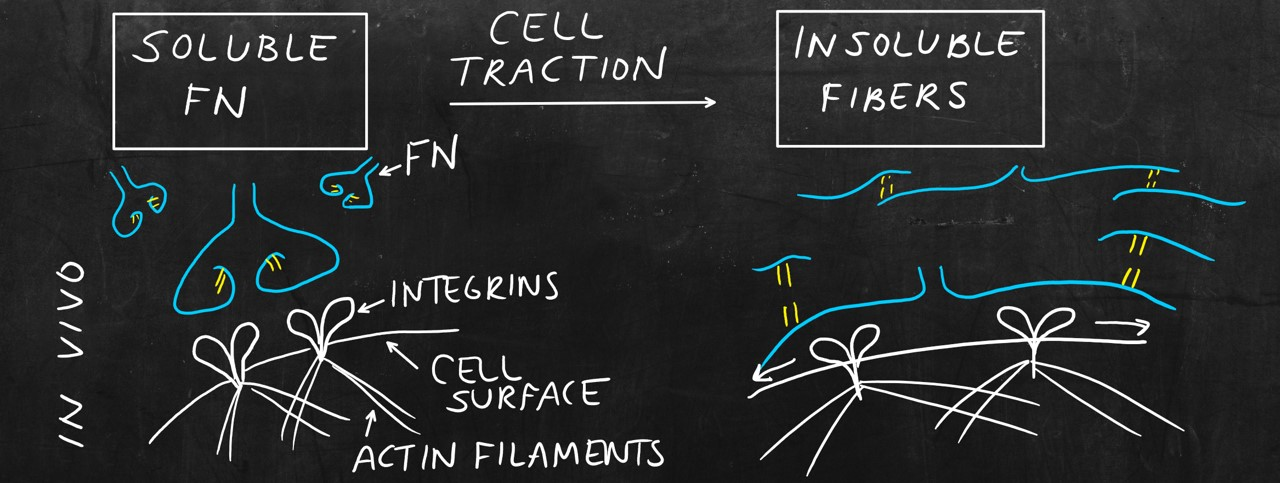
\includegraphics[width=\textwidth]{golecki_figure_1}
  \end{center}
  \caption{FN structure and unfolding in vivo. Schematic of the mechanism of FN fibrillogenesis.}
\end{figure}

To engineer fibrillar FN, we must first understand how it is built in vivo. Soluble,
globular FN circulates in the blood. Cells attach to FN via integrin binding receptors that transfer
mechanical traction forces to unfold FN. This unfolding exposes cryptic binding sites inducing
fibrillogenesis (Figure 1). The challenge is to replicate that process outside the body, turning fibrillogenesis into a manufacturing process. We propose that a perforated reservoir rotating at
high speeds may propel protein solutions out of the reservoir orifice stretching, drying and
solidifying nanofibers. Within that process we hypothesized that shear forces within the reservoir
are capable of unfolding FN inducing fibrillogenesis on the benchtop. Herein we describe a fluid
dynamics model of shear induced fibrillogenesis using this system to manufacture FN nanofibers
for future use in wound dressings.

\noindent
\textbf{Shear Fluid Model}

To test this hypothesis, we developed a mathematical model that predicts how shear forces generated using a spinning orifice can be used to induce the high-throughput production of FN nanofibers. Others have probed single FN molecules to determine tensile forces required to unfold FN. We used Mohr’s circle \cite{gere} to determine the shear stress required to unfold FN by translating values from single molecule uniaxial tensile tests \cite{oberhauser} to shear. Mohr’s circle is a graphical representation of the relationship between principle and shear stress. We calculated 3.7 kPa as the minimum shear stress required to unfold a FN molecule. Next, to calculate the shear produced by a spinning orifice, we derived a model from Navier Stokes for the shear stress distribution through the diameter of the orifice.

\renewcommand{\thefigure}{2}
\begin{figure}[h]
  \begin{center}
    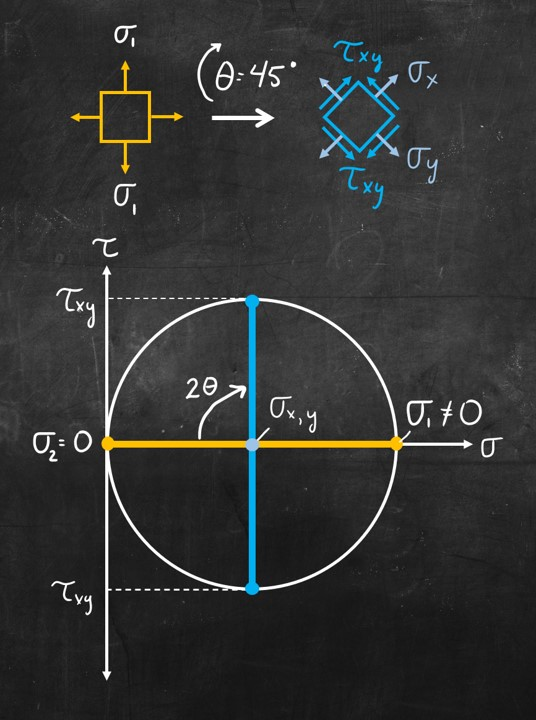
\includegraphics[scale=.55]{golecki_figure_2}
  \end{center}
  \caption{Mohr's circle for plane stress.}
\end{figure}

\renewcommand{\thefigure}{3}
\begin{figure}[h]
  \begin{center}
    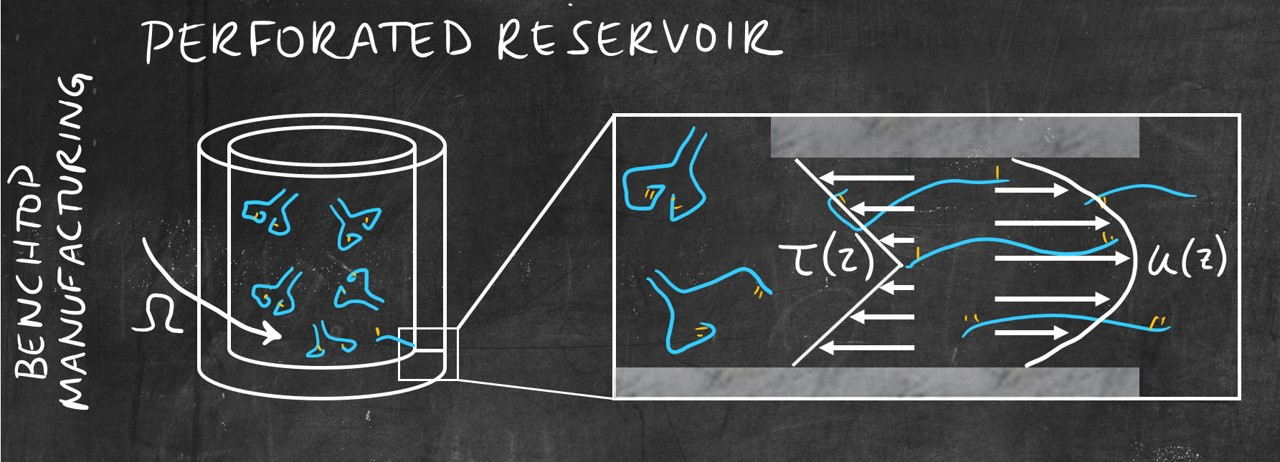
\includegraphics[scale=.5]{golecki_figure_3}
  \end{center}
  \caption{Schematic representing hypothesized benchtop shear unfolding in a rotating perforated reservoir.}
\end{figure}

\noindent
\textbf{Details of Shear Fluid Model}

To derive an equation of fluid flow through the orifice, we modeled shear stresses in a Poiseuille flow rotating with angular speed ($\Omega$). The system consists of a viscous, incompressible, fluid flowing through a tube of uniform cross section, rotating about the Y axis, applying the  following assumptions:

\begin{center}
1. The flow is steady and does not change with time: $\frac{du_z}{dt}=0$.\\
1a. Flow is in unidirectional: $u_r = 0; u_\theta = 0$.\\
2. The flow is axisymetric.
\end{center}

\renewcommand{\thefigure}{4}
\begin{figure}[h]
  \begin{center}
    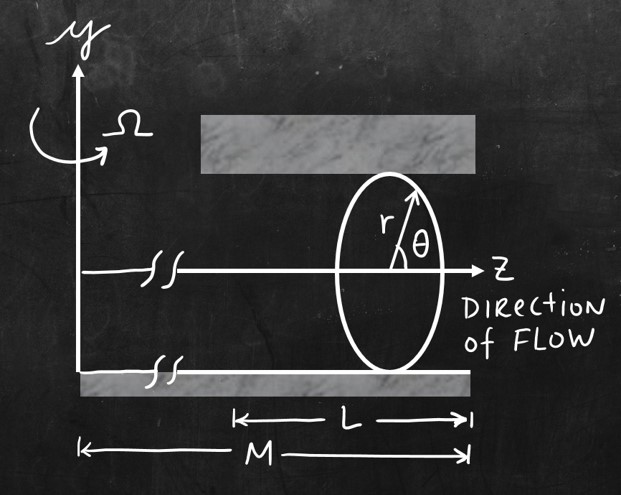
\includegraphics[scale=.42]{golecki_figure_4}
  \end{center}
  \caption{Schematic of reservoir orifice.}
\end{figure}

\noindent
\textit{Conservation of Mass (from the continuity equation):}
\[\frac{\partial}{\partial t}\rho 
+ \frac{1}{r}\frac{\partial r u_r}{\partial r}
+ \frac{1}{r}\frac{\partial r u_\theta}{\partial \theta}
+ \frac{\partial u_z}{\partial z}
= 0
\]

If density, $\rho$, does not change with time, there is no flow in the $r$ direction, then fluid speed does not change along the $z$ direction.
\[\frac{\partial u_z}{\partial z} = 0\]

\noindent
\textit{Conservation of Momentum:}

A very common case of Navier Stokes in cylindrical coordinates is axisymetric flow assuming no tangential velocity. The remaining quantities are independent of $\theta$. Therefore, N-S$_\theta$ goes to zero. Because we assume no flow in the $r$ direction, hydrostatic pressure is negligible, and $\frac{\partial u_z}{\partial z} = 0$ from continuity equation, N-S$_r$ goes to zero as well. From here, we study N-S in the $z$-direction:


\noindent
\textbf{References}
\begingroup
\renewcommand{\section}[2]{}% https://tex.stackexchange.com/questions/22645/hiding-the-title-of-the-bibliography
%\renewcommand{\chapter}[2]{}% for other classes
\begin{thebibliography}{3}
\bibitem{gere}
Gere, J. M. (2003). Mechanics of Materials: Thompson-Engineering.

\bibitem{oberhauser}
Oberhauser, A. F., Badilla-Fernandez, C., Carrion-Vazquez, M., and Fernandez, J. M. (2002).
The mechanical hierarchies of fibronectin observed with single-molecule AFM. 
\textit{Journal of Molecular Biology}, 319(2), 433-447. doi:10.1016/s0022-2836(02)00306-6

\bibitem{sawicka}
Sawicka, K. M., Seeliger, M., Musaev, T., Macri, L. K., and Clark, R. A. (2015). Fibronectin
interaction and enhancement of growth factors: importance for wound healing. 
\textit{Advances in wound care}, 4(8), 469-478.

\end{thebibliography}

\newpage

\nnwallpaper{2020_Intro_Section_Page_Border.pdf}

\begin{figure}[H]
    \centering
    \vspace*{50pt}
    
\includegraphics[scale=1.25]{newtons_notebook_fibonacci_spiral.png}
    \vspace*{25pt}
\end{figure}

    This issue of the \textit{Notebook} included submissions from our own students and faculty as well as alumni and friends of the Haverford community outside the walls of Wilson Hall. Also added in this issue were two new sections containing more complex articles with advanced arguments. The \textit{Notebook} team hopes that the increasing diversity of this journal inspires its readers to pursue STEM with unremitting fervor and renewed dedication. 

\begin{quotation}
\textit{We are at the very beginning of time for the human race. It is not unreasonable that we grapple with problems. But there are tens of thousands of years in the future. Our responsibility is to do what we can, learn what we can, improve the solutions, and pass them on.}
	\begin{flushright}
$\sim$Richard P. Feynman
	\end{flushright}
\end{quotation}

\begin{center}
If you are interested in contributing to the 2020-2021 edition of \textit{Newton’s Notebook},\\ 
please contact Gary Gao or Safa Obuz, Editors-in-Chief for Issue V.
\end{center}

% v COMMENT THIS OUT BEFORE SENDING THE FINAL VERSION TO PRINT, THEY DON'T WANT THE COVERS
\newpage
\nnimagepage{2020_Back_Cover.pdf}

\end{document}
